
\documentclass[11pt]{article}
\usepackage[a4paper,margin=1in]{geometry}
\usepackage{lmodern}
\usepackage[T1]{fontenc}
\usepackage[utf8]{inputenc}
\usepackage{amsmath,amssymb,amsthm}
\usepackage{mathtools}
\usepackage{microtype}
\usepackage{graphicx}
\usepackage{booktabs}
\usepackage{tabularx}
\usepackage{array}
\usepackage{xcolor}
\usepackage{float}
\usepackage{caption}
\usepackage{enumitem}
\usepackage{titlesec}
\usepackage[colorlinks=true,linkcolor=blue!50!black,urlcolor=blue!50!black,citecolor=blue!50!black]{hyperref}
\usepackage{siunitx}
\sisetup{detect-all}

\titleformat{\section}{\Large\bfseries\sffamily}{\thesection}{0.6em}{}
\titleformat{\subsection}{\large\bfseries\sffamily}{\thesubsection}{0.6em}{}
\titleformat{\subsubsection}{\normalsize\bfseries\sffamily}{\thesubsubsection}{0.6em}{}

\newcommand{\code}[1]{\texttt{#1}}
\setlength{\parskip}{0.4em}

\title{\textsf{\Huge Placement Pipeline}\\[0.3em]\textsf{\Large Visualization Report}}
\author{NestingRL --- Placement Network}
\date{\today}

\begin{document}
\maketitle

\begin{center}
\small
Checkpoint: \texttt{checkpoints/perthet\_combined/final.pt}\\[0.3em]
12 convex val pairs (orig\_idx $\in [10800, 12000)$),
6 concave-fs val pairs (\code{bo\_train\_pool\_10k} position $\in [9000, 10000)$).\\
Refinement window: $\pm10$\,px $\times \pm2$\,$\theta$-bins
$\Rightarrow$ 2205 Shapely calls per pair.
\end{center}

\tableofcontents
\newpage

\section{Placement Network --- Methodology}

A learned placement function that, given a free-space polygon $F$ and a part polygon $P$, returns a placement $(\theta, x, y)$ maximizing a Shapely-defined reward.  Trained on 22\,000 pairs (12\,k convex--convex + 10\,k concave-fs--convex), achieves val recovery $\approx 0.72$ with one small U-Net and one feed-forward pass per rotation.

\subsection{Formal problem statement}

\subsubsection{Notation}

Let
\begin{itemize}[leftmargin=*,nosep]
  \item $F \subset \mathbb{R}^2$ be a simple polygon (the \emph{free space}), possibly non-convex.
  \item $P \subset \mathbb{R}^2$ be a simple convex polygon (the \emph{part}), centered at the origin so that its centroid coincides with $(0,0)$.
  \item $R_\theta : \mathbb{R}^2 \to \mathbb{R}^2$ denote rotation by angle $\theta$ about the origin.
  \item $T_{(x,y)}$ denote translation by $(x,y)$.
  \item The \emph{placement} of $P$ at position $(x,y)$ with rotation $\theta$ is the set
  \[
    P_{\theta,x,y} \;=\; T_{(x,y)}\bigl(R_\theta(P)\bigr).
  \]
\end{itemize}

We discretize:
\begin{itemize}[leftmargin=*,nosep]
  \item Rotations: $\theta \in \Theta = \{0, \tfrac{2\pi}{36}, \tfrac{4\pi}{36}, \dots, \tfrac{70\pi}{36}\}$, indexed $i = 0, \dots, 35$.
  \item Positions: $(x,y) \in [-1,1]^2$ on a $128 \times 128$ raster grid. Each grid cell is indexed by row $r \in \{0, \dots, 127\}$ and column $c \in \{0, \dots, 127\}$. The pixel-to-world map is
  \[
    \operatorname{pix}^{-1}(r, c) \;=\; \left(\,\tfrac{2c}{127} - 1,\;\; 1 - \tfrac{2r}{127}\,\right) \in [-1,1]^2,
  \]
  so column $c$ is the $x$-axis (left $\to$ right) and row $r$ is the $y$-axis (top $\to$ bottom, sign-flipped to match image convention). Total pixels $\lvert\Omega\rvert = 128^2 = 16\,384$.
\end{itemize}

The full discrete action space has size $\lvert\Theta\rvert \cdot \lvert\Omega\rvert = 36 \cdot 16\,384 = 589\,824$.

\subsubsection{Validity and reward}

Define the \textbf{Inner Fit Polygon} at rotation $\theta$ as the locus of valid centroid positions:
\[
  \operatorname{IFP}(F, P, \theta) \;=\; \{ (x,y) \in \mathbb{R}^2 : P_{\theta,x,y} \subseteq F \}.
\]
Equivalently, $\operatorname{IFP}(F, P, \theta) = F \ominus R_\theta(P)$ (Minkowski erosion). It is well-defined and computable for any $F$ (convex or concave) and convex $P$.

\paragraph{Contact and reward functions}
For a free-space polygon $F$ and a placed-part polygon $Q \subseteq F$, define the \textbf{contact score}
\[
  \operatorname{contact}(F, Q) \;=\; \alpha\,\operatorname{adherence}(F, Q) \;+\; \beta\,\operatorname{proximity}(F, Q) \;+\; \gamma,
\]
where each term is normalized to lie in $[0, 1]$:
\begin{itemize}[leftmargin=*,nosep]
  \item \textbf{Adherence.} Fraction of $Q$'s perimeter that lies within $\varepsilon$ of $F$'s boundary:
  \[
    \operatorname{adherence}(F, Q) \;=\; \frac{\mathcal{H}^1\!\left(\{x \in \partial Q : \operatorname{dist}(x, \partial F) \leq \varepsilon\}\right)}{\mathcal{H}^1(\partial Q)},
  \]
  where $\mathcal{H}^1$ is 1-dimensional Hausdorff measure (arc-length) and $\partial$ denotes polygon boundary. We use $\varepsilon = 5 \cdot 10^{-3}$ in normalized $[-1,1]$ coordinates.
  \item \textbf{Proximity.} Mean closeness of $Q$'s perimeter to $\partial F$, with an exponential decay:
  \[
    \operatorname{proximity}(F, Q) \;=\; \frac{1}{\mathcal{H}^1(\partial Q)} \int_{\partial Q} \exp\!\left(-\frac{\operatorname{dist}(x, \partial F)}{\tau}\right) \, d\mathcal{H}^1(x),
  \]
  with characteristic length $\tau = 0.05$.
\end{itemize}

Weights $(\alpha, \beta, \gamma) = (0.5, 0.2, 0.3)$ are fixed; defined in \code{src/geometry/rewards.py::compute\_reward}.  By construction $\operatorname{contact}(F, Q) \in [\gamma, \gamma + \alpha + \beta] = [0.3, 1.0]$ for any $Q \subseteq F$.

The \textbf{scalar reward} at a placement is
\[
  r(F, P, \theta, x, y) \;=\;
  \begin{cases}
    \exp\!\left(k \cdot \operatorname{contact}(F, P_{\theta,x,y})\right) & \text{if } (x,y) \in \operatorname{IFP}(F,P,\theta) \\
    0 & \text{otherwise}
  \end{cases}
\]
where $k = 10$ is a sharpening constant.  The exponentiation turns additive contact differences into multiplicative reward differences, so the softmax-normalized heatmap (Section~\ref{sec:target}) concentrates mass near the best-contact placements.

\paragraph{Reward heatmap $H_\theta$}
For fixed $(F, P, \theta)$, define the discrete reward heatmap as the function
\[
  H_\theta : \{0, \dots, 127\}^2 \to \mathbb{R}_{\geq 0}, \qquad H_\theta[r, c] \;=\; r\!\left(F,\; P,\; \theta,\; \operatorname{pix}^{-1}(r, c)\right).
\]
Concretely, $H_\theta[r, c]$ is the reward of placing $R_\theta(P)$ with its centroid at world coordinates
\[
  \operatorname{pix}^{-1}(r, c) \;=\; \left(\frac{2c}{127} - 1,\;\; 1 - \frac{2r}{127}\right) \in [-1, 1]^2.
\]
Properties:

\begin{center}
\begin{tabular}{ll}
  \toprule
  property & value \\
  \midrule
  Tensor shape                & $128 \times 128$ \\
  Support                     & rasterized $\operatorname{IFP}(F, P, \theta) \cap \operatorname{pix}^{-1}(\{0,\dots,127\}^2)$ \\
  Range on support            & $[\exp(0.3 k),\, \exp(k)] = [\exp(3),\, \exp(10)] \approx [20,\, 22\,026]$ \\
  Range outside support       & $\{0\}$ \\
  Stacked over 36 rotations   & $\mathbf{H} \in \mathbb{R}_{\geq 0}^{36 \times 128 \times 128}$ \\
  \bottomrule
\end{tabular}
\end{center}

The full per-pair reward tensor is $\mathbf{H} = (H_{\theta_0}, \dots, H_{\theta_{35}})$, computed once per pair in the precompute stage and stored as float16 in the training pkl.  The brute-force optimum is $r^\ast = \max_{i,r,c} \mathbf{H}[i, r, c]$.

\subsubsection{Optimization objective}

The brute-force optimum for a pair is
\[
  (\theta^\ast, x^\ast, y^\ast) \;=\; \arg\max_{(\theta, x, y) \in \Theta \times \Omega} \; r(F, P, \theta, x, y),
  \qquad r^\ast = r(F, P, \theta^\ast, x^\ast, y^\ast).
\]
Computing it requires evaluating Shapely on every valid pixel --- too expensive for inference.  The placement network $\pi_\phi$ instead predicts a near-optimal placement in a single forward pass per rotation.

\subsubsection{Quality metric}

For a predicted placement $(\hat\theta, \hat x, \hat y)$:
\[
  \operatorname{recovery} \;=\; \frac{r(F, P, \hat\theta, \hat x, \hat y)}{r^\ast} \;\in\; [0, 1].
\]
We report mean recovery on a 2200-pair validation set.

\subsection{Model}

\subsubsection{Inputs}

For a given query rotation $\theta_i$:
\begin{itemize}[leftmargin=*,nosep]
  \item $\mathbf{m}_F \in \{0,1\}^{128\times128}$: rasterized free-space mask.
  \item $\mathbf{m}_{P,\theta_i} \in \{0,1\}^{128\times128}$: rasterized mask of $R_{\theta_i}(P)$, with its centroid placed at the image center.
\end{itemize}
Stacked: $\mathbf{x}_i = \operatorname{stack}(\mathbf{m}_F, \mathbf{m}_{P,\theta_i}) \in \mathbb{R}^{2\times128\times128}$.

\subsubsection{Architecture: $\pi_\phi$}

A 4-level U-Net (\code{\_SmallUNet} in \code{src/models/neural\_bo\_policy.py}):
\[
  \pi_\phi : \mathbb{R}^{2\times128\times128} \to \mathbb{R}^{128\times128}.
\]

\paragraph{Building blocks}
Let $C \in \mathbb{R}^{c_{\text{in}} \times H \times W}$ denote a tensor with $c_{\text{in}}$ channels at spatial resolution $H \times W$.

\textbf{(a) ConvBlock} $\mathcal{C}_{c_{\text{out}}}$.  Two stacked stages of ($3{\times}3$ conv with same-padding, BatchNorm2d, ReLU):
\[
  \mathcal{C}_{c_{\text{out}}}(C) \;=\; \operatorname{ReLU}\!\left(\operatorname{BN}\!\left(W_2 \star \operatorname{ReLU}\!\left(\operatorname{BN}\!\left(W_1 \star C\right)\right)\right)\right),
\]
where $W_1 \in \mathbb{R}^{c_{\text{out}}\times c_{\text{in}}\times 3\times 3}$, $W_2 \in \mathbb{R}^{c_{\text{out}}\times c_{\text{out}}\times 3\times 3}$, and $\star$ denotes 2D convolution with padding 1 (output preserves $H, W$).

\textbf{(b) Down}: max-pool with stride 2:
\[
  \operatorname{Down}(C) \in \mathbb{R}^{c_{\text{in}}\times H/2 \times W/2}, \qquad
  \operatorname{Down}(C)[c, i, j] = \max_{a,b\in\{0,1\}} C[c,\, 2i+a,\, 2j+b].
\]

\textbf{(c) Up}: bilinear upsample by factor 2:
\[
  \operatorname{Up}(C) \in \mathbb{R}^{c_{\text{in}}\times 2H \times 2W}.
\]

\textbf{(d) SkipCat}: channel-wise concatenation with the corresponding encoder feature at matched resolution:
\[
  \operatorname{SkipCat}(U, E) \;=\; [U;\,E] \;\in\; \mathbb{R}^{(c_U+c_E)\times H \times W}.
\]

\paragraph{Forward pass}
With base width $b = 32$:

\textbf{Encoder.}
\[
\begin{aligned}
e_1 &= \mathcal{C}_{b}(\mathbf{x}_i)            && \in\,\mathbb{R}^{32\times128\times128}\\
e_2 &= \mathcal{C}_{2b}(\operatorname{Down}(e_1))     && \in\,\mathbb{R}^{64\times64\times64}\\
e_3 &= \mathcal{C}_{4b}(\operatorname{Down}(e_2))     && \in\,\mathbb{R}^{128\times32\times32}\\
e_4 &= \mathcal{C}_{8b}(\operatorname{Down}(e_3))     && \in\,\mathbb{R}^{256\times16\times16}
\end{aligned}
\]

\textbf{Bottleneck.}
\[
  g \;=\; \mathcal{C}_{8b}(e_4) \;\in\;\mathbb{R}^{256\times16\times16}.
\]

\textbf{Decoder.} (mirror of encoder, with skip concatenation)
\[
\begin{aligned}
d_3 &= \mathcal{C}_{4b}\!\left(\operatorname{SkipCat}(\operatorname{Up}(g),\,e_3)\right)   && \in\,\mathbb{R}^{128\times32\times32}\\
d_2 &= \mathcal{C}_{2b}\!\left(\operatorname{SkipCat}(\operatorname{Up}(d_3),\,e_2)\right) && \in\,\mathbb{R}^{64\times64\times64}\\
d_1 &= \mathcal{C}_{b}\!\left(\operatorname{SkipCat}(\operatorname{Up}(d_2),\,e_1)\right)  && \in\,\mathbb{R}^{32\times128\times128}
\end{aligned}
\]

\textbf{Output head.}  $1{\times}1$ convolution to a single channel:
\[
  \mathbf{z}_i \;=\; W_{\text{out}} \star d_1 \;\in\; \mathbb{R}^{1\times128\times128},
\]
with $W_{\text{out}} \in \mathbb{R}^{1\times32\times1\times1}$.  Squeezing the singleton channel gives $\mathbf{z}_i \in \mathbb{R}^{128\times128}$, the per-pixel logit map for rotation $\theta_i$.

\paragraph{Receptive field and parameter count}
Receptive field at the bottleneck spans the full input ($e_4$ has spatial $16{\times}16$ covering $128{\times}128$ -- each bottleneck cell ``sees'' all of the input through the 4-level downsampling). This is necessary because the optimum placement depends on global free-space geometry, not just local pixel neighborhoods.

Parameter table (with $b = 32$, $K = 9$ being the kernel-element count for a $3{\times}3$ conv):

\begin{center}
\begin{tabular}{lr}
  \toprule
  stage & params (approx) \\
  \midrule
  $\mathcal{C}_b$ on $c_\text{in}=2$           & $2 \cdot b \cdot K + b \cdot b \cdot K = 9\,792$ \\
  $\mathcal{C}_{2b}$ on $b$                    & $b \cdot 2b \cdot K + 2b \cdot 2b \cdot K = 55\,296$ \\
  $\mathcal{C}_{4b}$ on $2b$                   & $2b \cdot 4b \cdot K + 4b \cdot 4b \cdot K = 221\,184$ \\
  $\mathcal{C}_{8b}$ on $4b$                   & $4b \cdot 8b \cdot K + 8b \cdot 8b \cdot K = 884\,736$ \\
  Bottleneck $\mathcal{C}_{8b}$ on $8b$        & $8b \cdot 8b \cdot K + 8b \cdot 8b \cdot K = 1\,179\,648$ \\
  Decoder $\mathcal{C}_{4b}$ on $8b+4b$        & $12b \cdot 4b \cdot K + 4b \cdot 4b \cdot K = 663\,552$ \\
  Decoder $\mathcal{C}_{2b}$ on $4b+2b$        & $6b \cdot 2b \cdot K + 2b \cdot 2b \cdot K = 165\,888$ \\
  Decoder $\mathcal{C}_{b}$ on $2b+b$          & $3b \cdot b \cdot K + b \cdot b \cdot K = 36\,864$ \\
  Output $1{\times}1$ conv: $b \to 1$          & $32 + 1 = 33$ \\
  BatchNorm affines + biases (small)           & $\sim 6\,000$ \\
  \midrule
  \textbf{Total}                               & $\approx 3.13 \times 10^6$ \\
  \bottomrule
\end{tabular}
\end{center}

\subsubsection{Why this conditioning works}

The model never has to \emph{infer} rotation from the un-rotated part.  Conditioning the input on $\theta_i$ via $\mathbf{m}_{P,\theta_i}$ collapses the prediction task into a translation-equivariant question: ``given this oriented part and this free space, where does it fit best?'' This is the standard inductive bias of a U-Net.

\subsection{Training objective}

\subsubsection{Target distribution}\label{sec:target}

For each $(F, P, \theta_i)$ training example, define the \emph{normalized soft target}
\[
  \tilde{H}_{\theta_i}[r,c] \;=\; \frac{H_{\theta_i}[r,c]}{\sum_{r',c'} H_{\theta_i}[r',c']}.
\]
Since the precomputed $H_{\theta_i}$ uses $r = \exp(k \cdot \operatorname{contact})$, $\tilde{H}_{\theta_i}$ is a temperature-$1/k$ softmax of the underlying contact field over the IFP.

\subsubsection{Loss}

Let $\mathbf{p}_i = \operatorname{softmax}(\mathbf{z}_i) \in \Delta^{16383}$ (softmax over the 16\,384 flattened pixels).  The per-example soft cross-entropy loss is
\[
  \mathcal{L}_i(\phi) \;=\; -\sum_{r,c} \tilde{H}_{\theta_i}[r,c] \, \log \mathbf{p}_i[r,c].
\]
Equivalently, $\mathcal{L}_i = D_{\operatorname{KL}}(\tilde H_{\theta_i} \,\|\, \mathbf{p}_i) + \operatorname{H}(\tilde H_{\theta_i})$, where the entropy term is an example-dependent constant.

Compared to hard-label CE (one-hot at $\arg\max$), the soft loss provides gradient on every cell weighted by reward, which empirically lifts val recovery from $0.43 \to 0.72$ in our experiments.

\subsubsection{Training-step distribution}

Let $\mathcal{D} = \{(F_j, P_j, H^{(j)})\}_{j=1}^{N}$ be the corpus of $N = 22\,000$ training pairs (each with its 36-rotation heatmap tensor).  Sampling for each SGD step:
\[
  j \sim \operatorname{Uniform}\{1, \dots, N\}, \qquad i \sim \operatorname{Uniform}\{0, \dots, 35\},
\]
and the per-step empirical objective is $\mathbb{E}_{j,i}[\mathcal{L}_{i}(\phi; F_j, P_j)]$.  Roughly $N \cdot 36 = 7.92 \times 10^5$ distinct $(j, i)$ examples are addressable.

\subsubsection{Augmentation: dihedral group $D_2$}

Applied at the dataloader level.  Let $\sigma_h$ (horizontal flip) and $\sigma_v$ (vertical flip) act on the rasterized image plane.  Each is applied with probability $\tfrac12$, independently:
\begin{itemize}[leftmargin=*,nosep]
  \item $\sigma_h$: spatial axis-1 reversal; rotation reindex $i \mapsto (-i) \bmod 36$.
  \item $\sigma_v$: spatial axis-0 reversal; rotation reindex $i \mapsto (18 - i) \bmod 36$.
\end{itemize}

The transform is applied jointly to $(\mathbf{m}_F, \mathbf{m}_{P,\theta_i}, \tilde H_{\theta_i})$, preserving the input--target consistency.  Under reflection of the entire scene, the placement problem maps to itself, so the loss is unchanged in distribution.  Effective dataset multiplier: $\lvert D_2 \rvert = 4$.

\subsubsection{Optimization}

\begin{itemize}[leftmargin=*,nosep]
  \item Optimizer: AdamW, weight decay $10^{-4}$.
  \item Learning rate: $\eta_0 = 3 \times 10^{-4}$, cosine-annealed to 0 over $T = 8000$ steps.
  \item Batch size: 256.
  \item Mixed precision (FP16 amp).
  \item Hardware: Modal A100-80GB, $\sim 4.2$ steps/sec, $\sim 30$ min wall.
\end{itemize}

\subsection{Inference}\label{sec:inference}

For a deployment query on $(F, P)$:
\begin{enumerate}[leftmargin=*,nosep]
  \item Rasterize $\mathbf{m}_F$.
  \item For each $i \in \{0, \dots, 35\}$: rasterize $\mathbf{m}_{P,\theta_i}$, run $\mathbf{z}_i = \pi_\phi(\mathbf{x}_i)$.
  \item Stack: $\mathbf{Z} = [\mathbf{z}_0, \dots, \mathbf{z}_{35}] \in \mathbb{R}^{36\times128\times128}$.
  \item Predict $(\hat\imath, \hat r, \hat c) = \arg\max_{i,r,c} \mathbf{Z}[i,r,c]$, giving $\hat\theta = \theta_{\hat\imath}$, $(\hat x, \hat y) = \operatorname{pix}^{-1}(\hat r, \hat c)$.
  \item \textbf{Optional refinement.}  Evaluate Shapely reward on a local window
  \[
    \mathcal{W} \;=\; \left\{(\theta_{\hat\imath + \delta_\theta},\, \hat r + \delta_r,\, \hat c + \delta_c) : \lvert\delta_\theta\rvert \leq K,\ \lvert\delta_r\rvert, \lvert\delta_c\rvert \leq N\right\}
  \]
  and return $\arg\max_{\mathcal W} r(\cdot)$.  With $N = 10, K = 2$, $\lvert\mathcal{W}\rvert = 5 \cdot 21^2 = 2205$ Shapely calls at $\sim 75\,\mu s$ each $\approx 165$ ms.  Closes the model-vs-brute-force gap.
\end{enumerate}

Latency without refinement: 36 forward passes on a 3M-param U-Net, dominated by per-rotation Shapely-free rasterization $\sim 30$ ms total on a CPU; the pure model forward passes are $< 50$ ms on GPU.

\subsection{Data pipeline}

\subsubsection{Pair generation}
\begin{itemize}[leftmargin=*,nosep]
  \item \textbf{Convex--convex.}  Random convex hulls from $n$ uniform points; 12\,000 pairs sampled by \code{generate\_bc\_dataset.py}.
  \item \textbf{Concave-fs / convex-part.}  From \code{bo\_train\_pool\_10k.pkl}: 10\,000 pairs with non-convex $F$ (random star polygons) and convex $P$.
\end{itemize}

\subsubsection{IFP precompute}
For each pair and each $\theta_i$: compute $\operatorname{IFP}(F, P, \theta_i)$ via Minkowski erosion using \code{pyclipper} (\code{src/geometry/ifp.py}).  Rasterize to $\{0,1\}^{128\times128}$.

\subsubsection{Reward heatmap precompute}
For each pixel inside the rasterized IFP, evaluate $r(F, P, \theta_i, x, y)$ via Shapely.  Pixels outside IFP are 0.  Stored as $(36, 128, 128)$ float32 per pair.

Total Shapely queries: $\sim 7.1 \times 10^8$ for convex + $\sim 3.1 \times 10^8$ for concave $\approx 10^9$ queries.  Executed in parallel across 100 Modal containers $\times$ 8 cores.  Total wall $\approx 25$ minutes; cost $\approx \$40$.

\subsubsection{Rotated-part-mask precompute}
For each pair: rasterize $R_{\theta_i}(P)$ centered at origin, for $i = 0, \dots, 35$.  Stored as $(36, 128, 128)$ uint8 per pair.  Used as the second input channel at training and inference.

\subsubsection{Combined corpus}
$N_{\text{train}} = 19\,800$ pairs (10\,800 convex + 9\,000 concave), $N_{\text{val}} = 2\,200$ (1200 convex + 1000 concave).  Combined pkl: $26.68$ GB (fp16 heatmaps + uint8 masks).

\subsection{Results}

Model selection: best mean val recovery on a fixed 2200-pair validation set, evaluated every 250 steps.  Compare model-only recovery (no Shapely refine):

\begin{center}
\begin{tabular}{lr}
  \toprule
  Configuration & Val recovery \\
  \midrule
  Hard label, hierarchical (tile + cell)                          & 0.04 \\
  Soft label, hierarchical                                         & 0.43 \\
  Soft label, hierarchical, tile-only                              & 0.32 \\
  \textbf{Per-(pair, $\theta$) U-Net, convex-only ($N=10\,800$)}   & \textbf{0.72} \\
  \textbf{Per-(pair, $\theta$) U-Net, combined ($N=19\,800$)}      & \textbf{0.73} \\
  \bottomrule
\end{tabular}
\end{center}

The convex-only and combined models are nearly tied on a mixed val set; combined generalizes to concave free spaces from a single checkpoint.  With Shapely refinement, both push to near-$1.0$ recovery (analytically: refinement window contains the true argmax with high probability if the model lands within $\pm 10$ pixels and $\pm 2$ rotation bins).

\subsection{Implementation pointers}

\begin{center}
\begin{tabular}{ll}
  \toprule
  concern & file \\
  \midrule
  Model                          & \code{src/models/neural\_bo\_policy.py::\_SmallUNet} \\
  Training script                & \code{scripts/train\_perthet.py} \\
  Modal training entrypoint      & \code{modal\_train\_perthet.py} \\
  IFP exact (handles concave fs) & \code{src/geometry/ifp.py::compute\_ifp\_exact} \\
  Reward function                & \code{src/geometry/rewards.py::compute\_reward\_exp} \\
  Concave precompute             & \code{modal\_concave\_precompute.py} \\
  Combined-pkl build             & \code{modal\_build\_combined.py} \\
  Best ckpt --- convex           & \code{checkpoints/perthet/final.pt} \\
  Best ckpt --- combined         & \code{checkpoints/perthet\_combined/final.pt} \\
  \bottomrule
\end{tabular}
\end{center}

\newpage
\section{Examples --- Convex--convex pairs}
The free-space polygon and the part polygon are both convex.  Brute-force ground truth $r^\ast$ comes from precomputed heatmap chunks (\code{data/reward\_heatmaps\_exp\_k10\_inside.npy\_chunks/}). For each pair we show, top row left to right: the model's predicted reward map at $\hat\theta$ (with the refinement window outlined and the refined target circled), the brute-force ground-truth reward map at $\theta^\ast$, and the part polygon (centered).  Bottom row: the model-only placement, the placement after Shapely refinement, and the brute-force placement.

\subsection{Pair convex\_10819 \quad\small\textmd{(area ratio 0.214)}}

\begin{figure}[H]
\centering
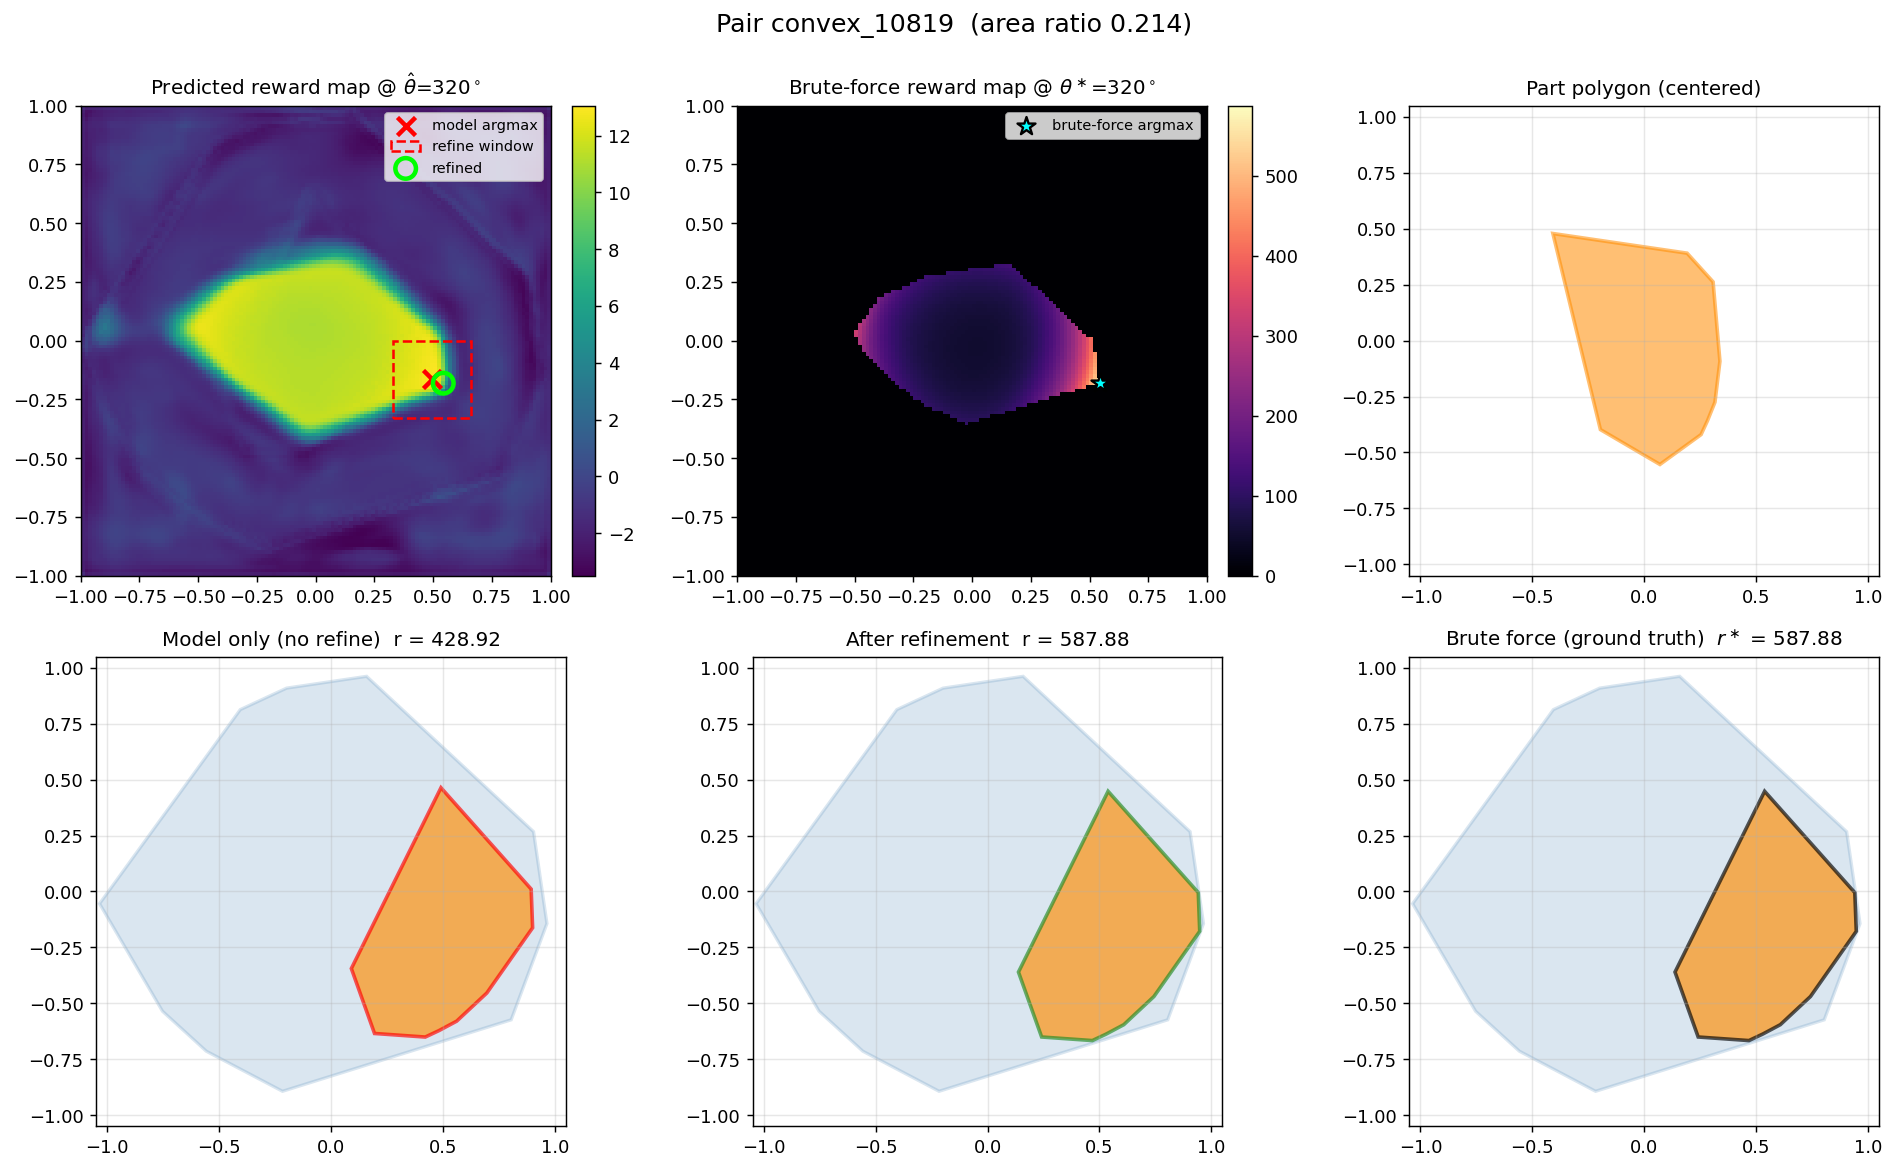
\includegraphics[width=\textwidth]{figs/convex_10819.png}
\end{figure}

\begin{center}\small
\begin{tabular}{lrrrr}
  \toprule
  Method & $\theta$ (deg) & $(x, y)$ & Reward & Recovery \\
  \midrule
  Brute force ($r^\ast$)    & 320 & $(+0.543, -0.181)$ & 587.882 & 1.000 \\
  Model only                & 320 & $(+0.496, -0.165)$       & 428.924 & 0.730 \\
  Refined ($\pm10$\,px, $\pm2$\,$\theta$-bins) & 320 & $(+0.543, -0.181)$ & 587.882 & 1.000 \\
  \bottomrule
\end{tabular}
\end{center}

\begin{center}\small
\begin{tabular}{lr}
  \toprule
  Cost & Value \\
  \midrule
  Rasterize (36 rotated part masks)              & 8.4 ms \\
  Model forward (36 passes, batched)             & 861.0 ms \\
  Shapely refinement (2205 calls, target 2205)  & 730.1 ms \\
  \midrule
  Total                                          & 1599.4 ms \\
  \bottomrule
\end{tabular}
\end{center}

\subsection{Pair convex\_10848 \quad\small\textmd{(area ratio 0.425)}}

\begin{figure}[H]
\centering
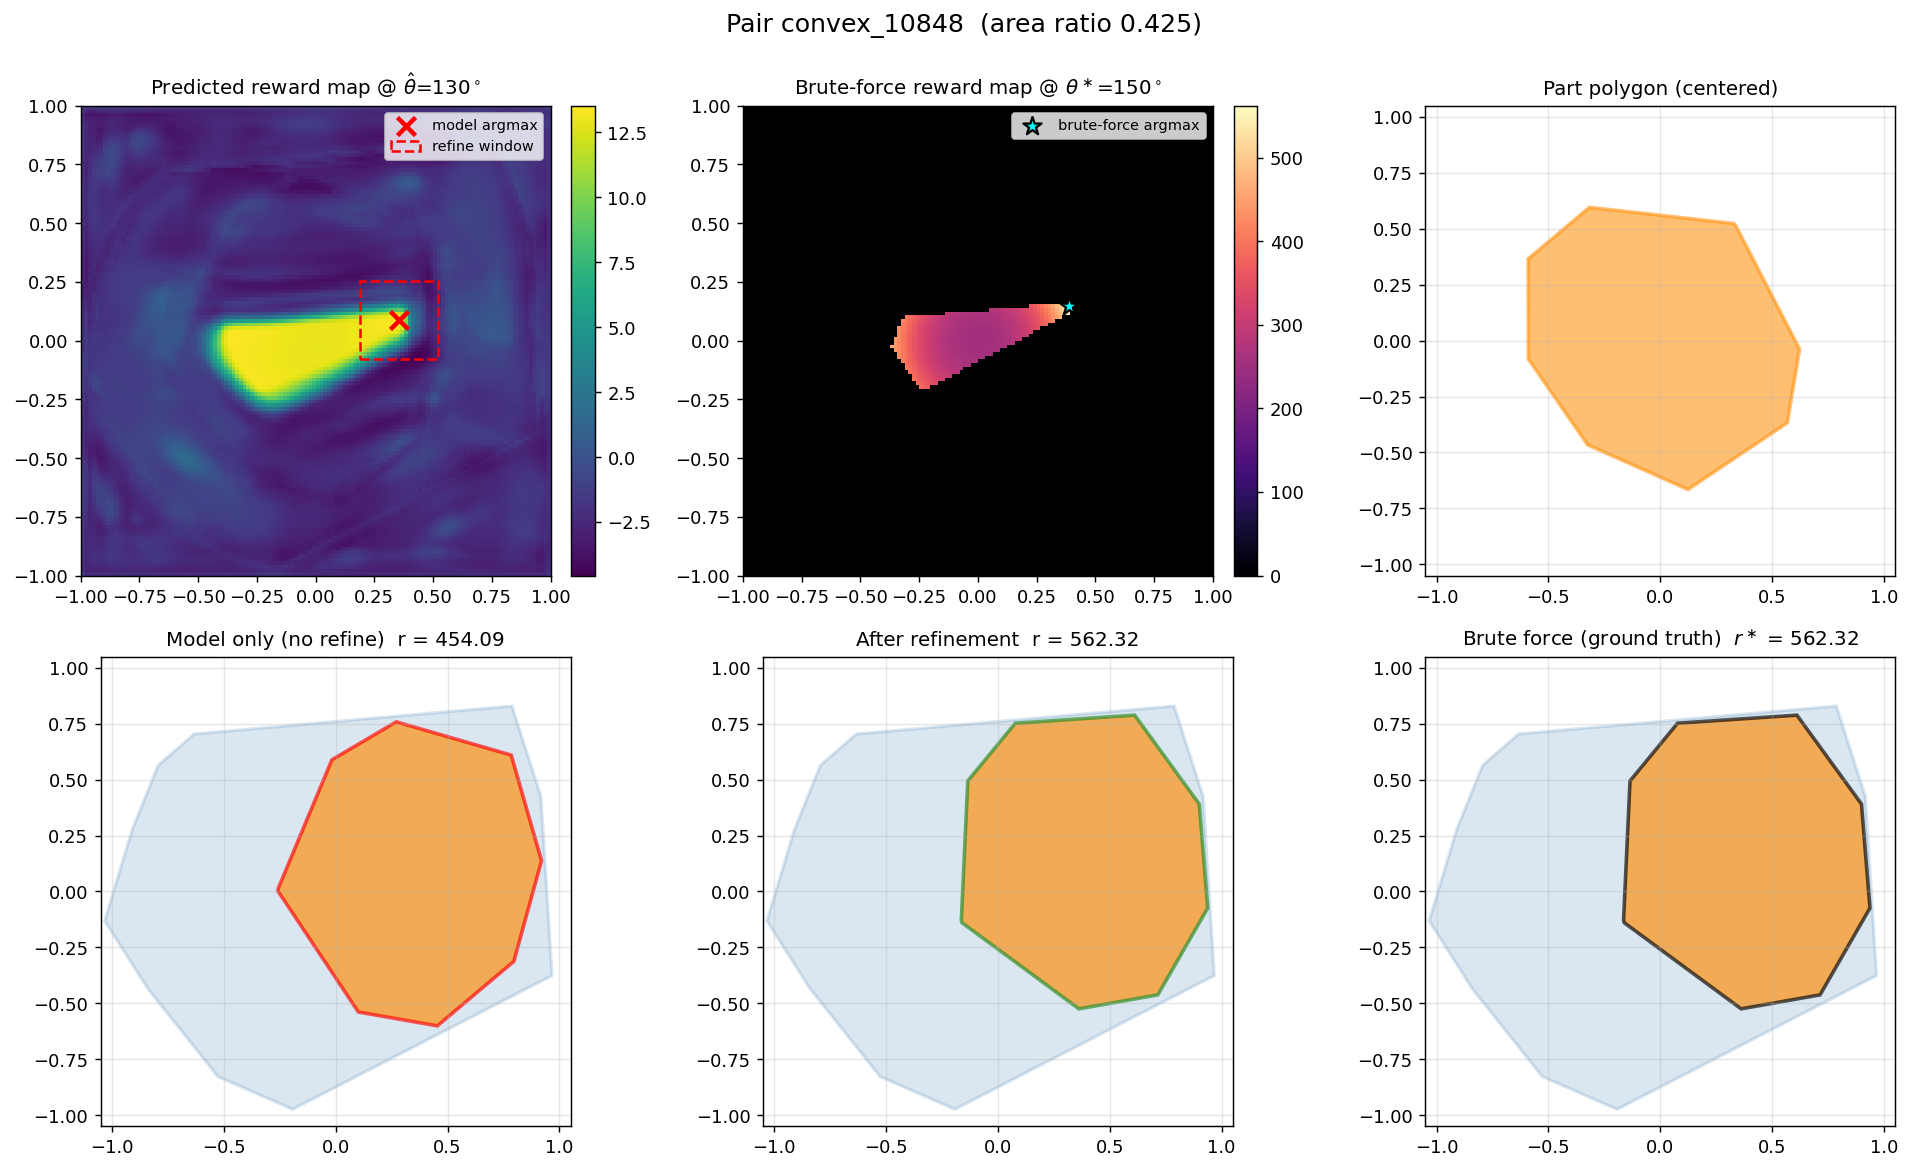
\includegraphics[width=\textwidth]{figs/convex_10848.png}
\end{figure}

\begin{center}\small
\begin{tabular}{lrrrr}
  \toprule
  Method & $\theta$ (deg) & $(x, y)$ & Reward & Recovery \\
  \midrule
  Brute force ($r^\ast$)    & 150 & $(+0.386, +0.150)$ & 562.316 & 1.000 \\
  Model only                & 130 & $(+0.354, +0.087)$       & 454.095 & 0.808 \\
  Refined ($\pm10$\,px, $\pm2$\,$\theta$-bins) & 150 & $(+0.386, +0.150)$ & 562.316 & 1.000 \\
  \bottomrule
\end{tabular}
\end{center}

\begin{center}\small
\begin{tabular}{lr}
  \toprule
  Cost & Value \\
  \midrule
  Rasterize (36 rotated part masks)              & 7.4 ms \\
  Model forward (36 passes, batched)             & 47.5 ms \\
  Shapely refinement (2205 calls, target 2205)  & 481.0 ms \\
  \midrule
  Total                                          & 535.9 ms \\
  \bottomrule
\end{tabular}
\end{center}

\subsection{Pair convex\_10889 \quad\small\textmd{(area ratio 0.468)}}

\begin{figure}[H]
\centering
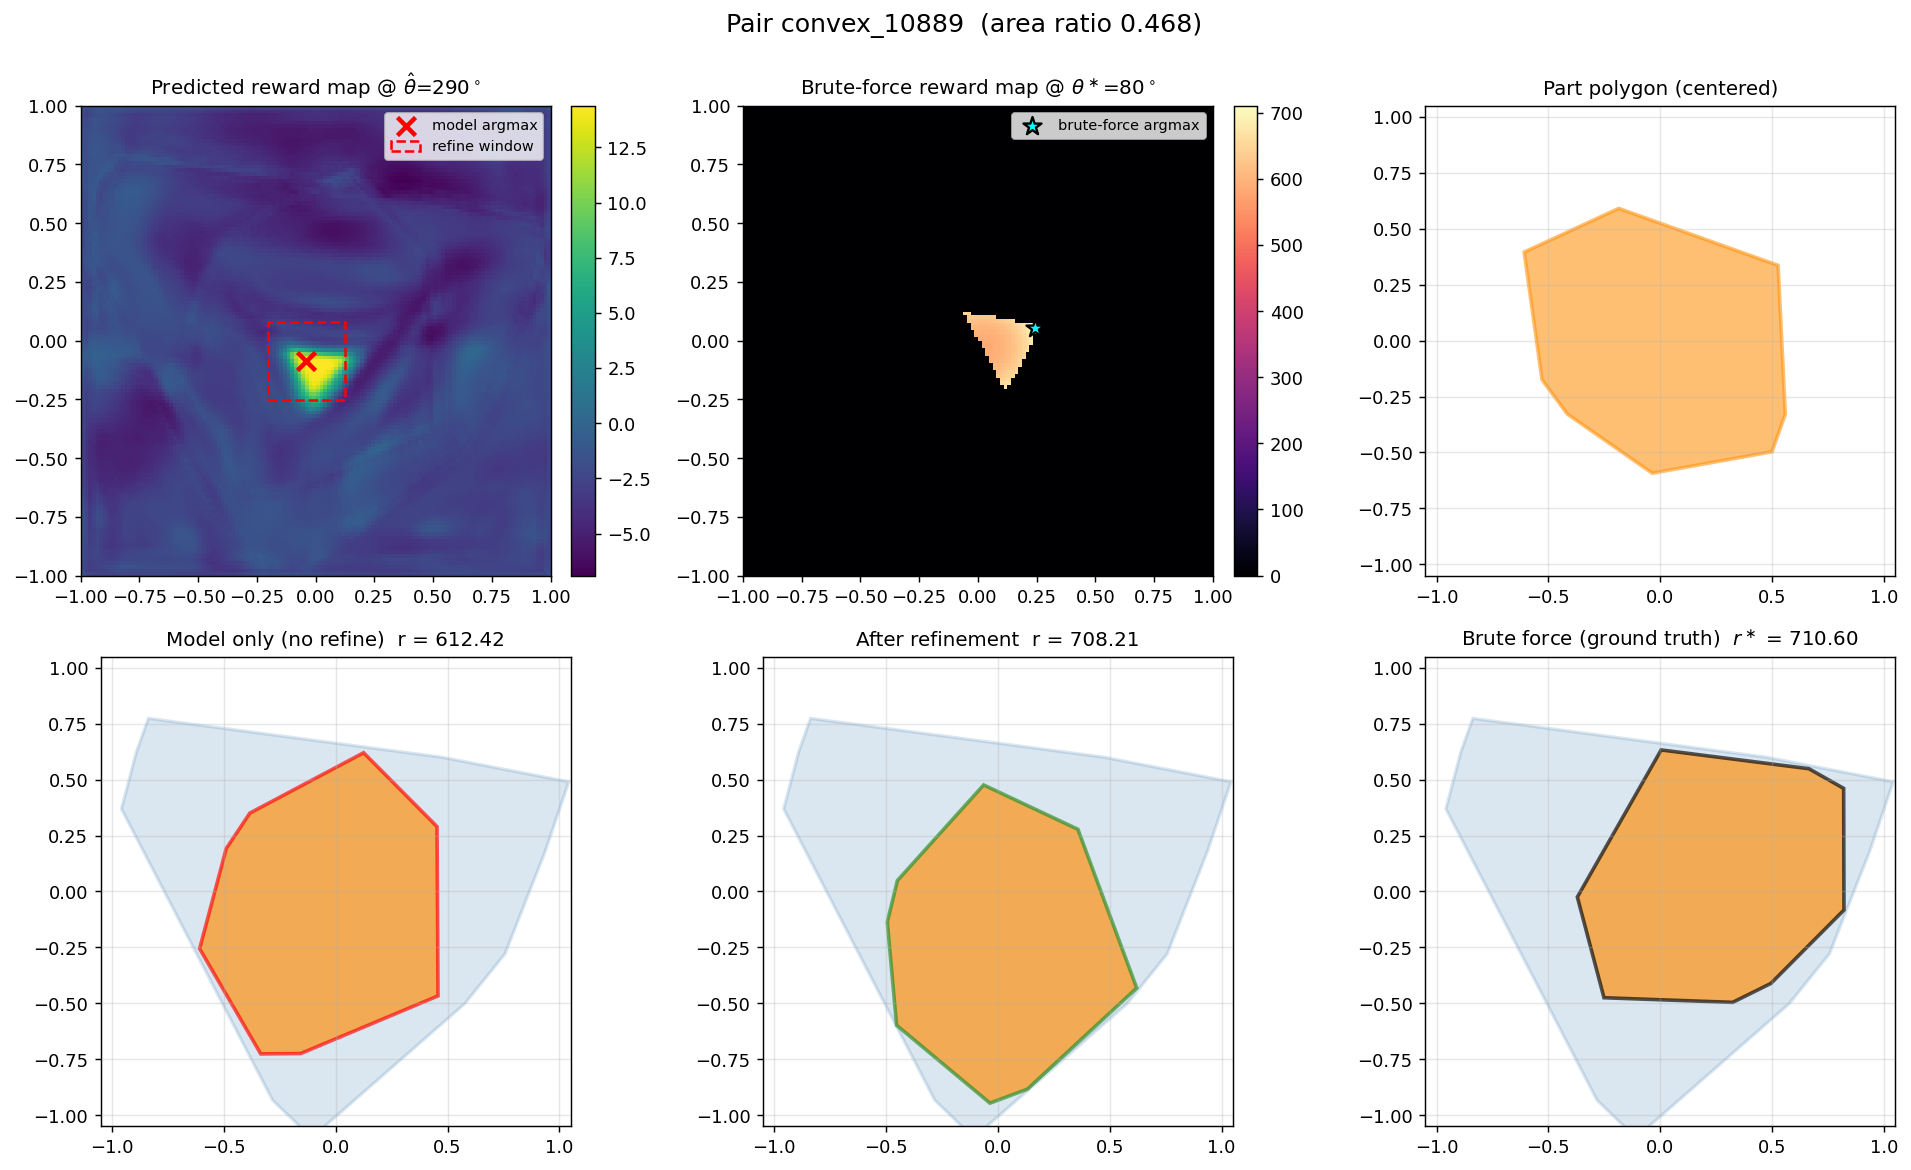
\includegraphics[width=\textwidth]{figs/convex_10889.png}
\end{figure}

\begin{center}\small
\begin{tabular}{lrrrr}
  \toprule
  Method & $\theta$ (deg) & $(x, y)$ & Reward & Recovery \\
  \midrule
  Brute force ($r^\ast$)    & 80 & $(+0.244, +0.055)$ & 710.603 & 1.000 \\
  Model only                & 290 & $(-0.039, -0.087)$       & 612.424 & 0.862 \\
  Refined ($\pm10$\,px, $\pm2$\,$\theta$-bins) & 310 & $(+0.024, -0.244)$ & 708.210 & 0.997 \\
  \bottomrule
\end{tabular}
\end{center}

\begin{center}\small
\begin{tabular}{lr}
  \toprule
  Cost & Value \\
  \midrule
  Rasterize (36 rotated part masks)              & 6.2 ms \\
  Model forward (36 passes, batched)             & 45.2 ms \\
  Shapely refinement (2205 calls, target 2205)  & 394.2 ms \\
  \midrule
  Total                                          & 445.6 ms \\
  \bottomrule
\end{tabular}
\end{center}

\subsection{Pair convex\_11009 \quad\small\textmd{(area ratio 0.140)}}

\begin{figure}[H]
\centering
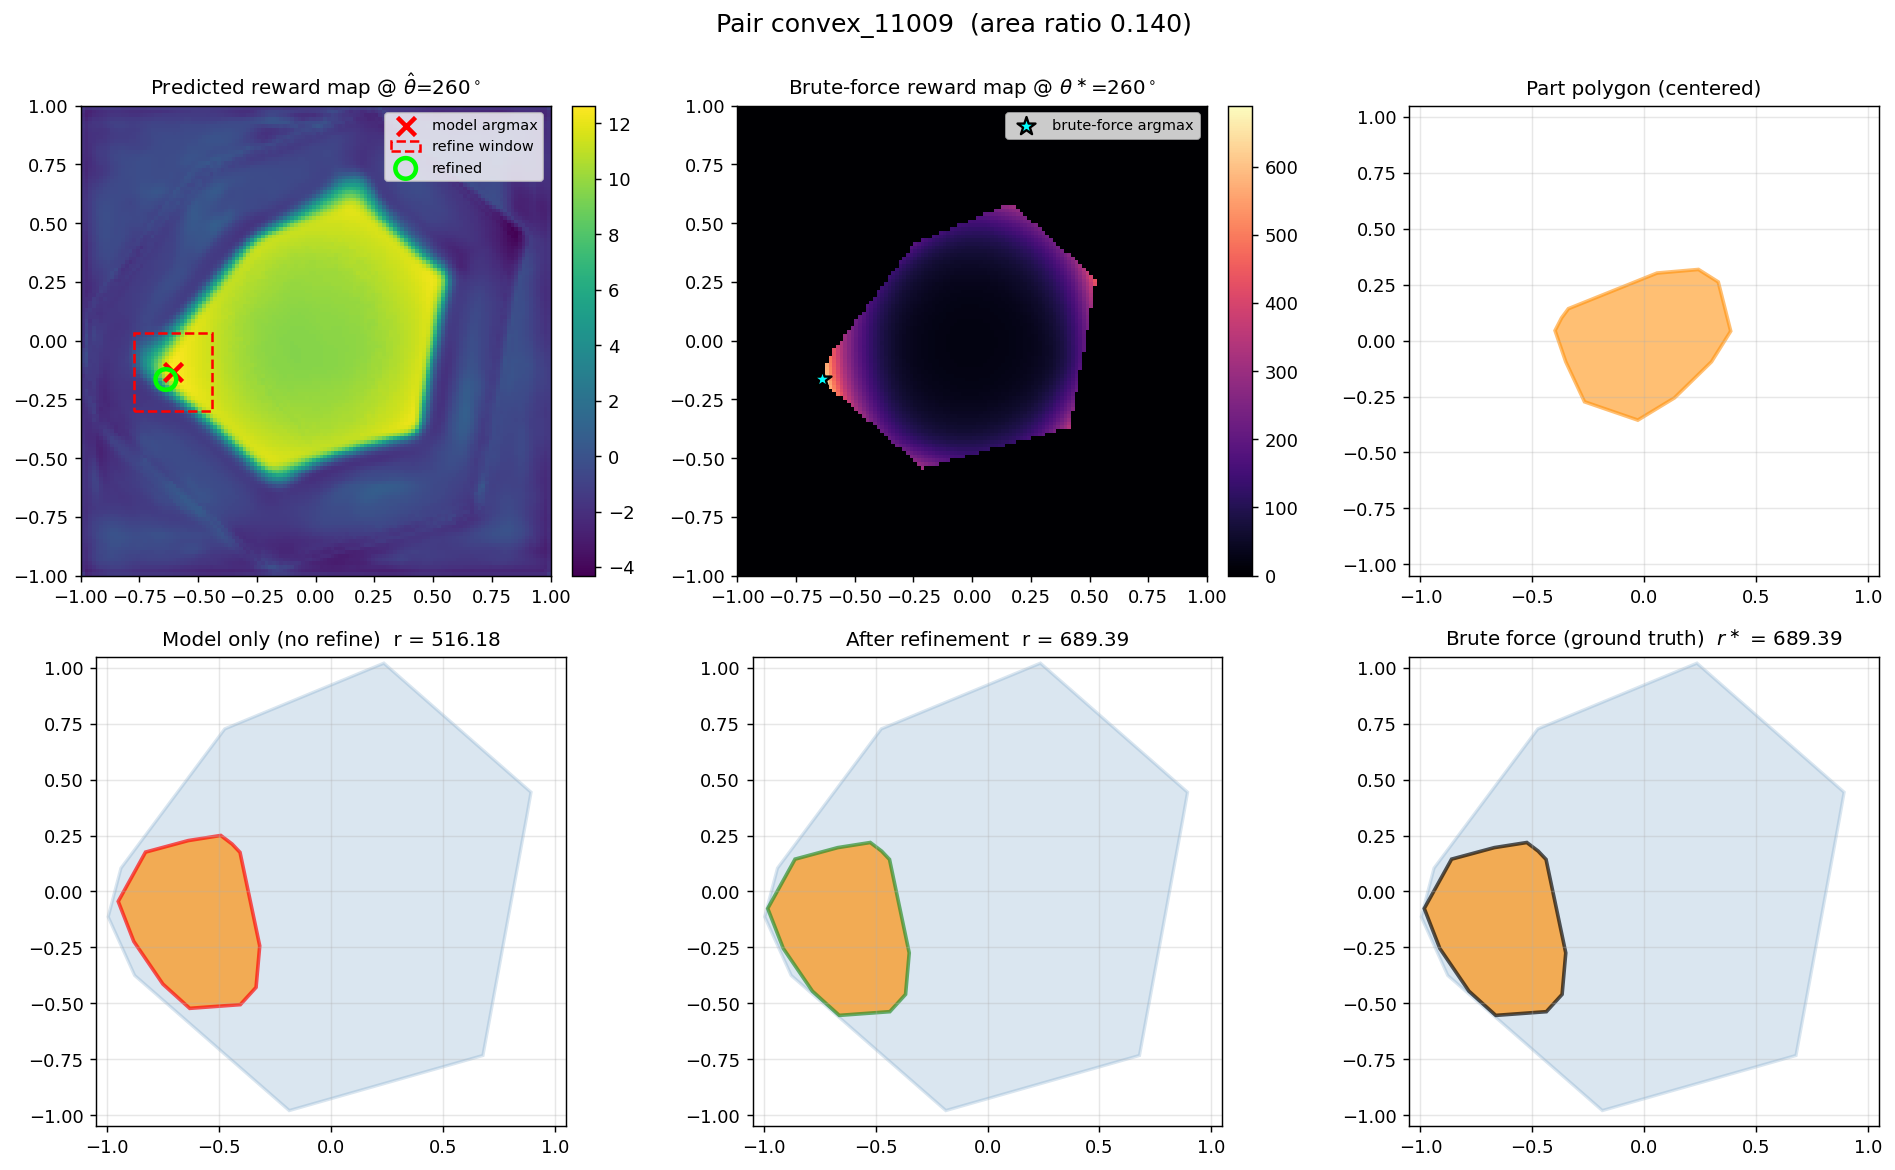
\includegraphics[width=\textwidth]{figs/convex_11009.png}
\end{figure}

\begin{center}\small
\begin{tabular}{lrrrr}
  \toprule
  Method & $\theta$ (deg) & $(x, y)$ & Reward & Recovery \\
  \midrule
  Brute force ($r^\ast$)    & 260 & $(-0.638, -0.165)$ & 689.395 & 1.000 \\
  Model only                & 260 & $(-0.606, -0.134)$       & 516.184 & 0.749 \\
  Refined ($\pm10$\,px, $\pm2$\,$\theta$-bins) & 260 & $(-0.638, -0.165)$ & 689.395 & 1.000 \\
  \bottomrule
\end{tabular}
\end{center}

\begin{center}\small
\begin{tabular}{lr}
  \toprule
  Cost & Value \\
  \midrule
  Rasterize (36 rotated part masks)              & 6.7 ms \\
  Model forward (36 passes, batched)             & 44.4 ms \\
  Shapely refinement (2205 calls, target 2205)  & 700.8 ms \\
  \midrule
  Total                                          & 752.0 ms \\
  \bottomrule
\end{tabular}
\end{center}

\subsection{Pair convex\_11121 \quad\small\textmd{(area ratio 0.059)}}

\begin{figure}[H]
\centering
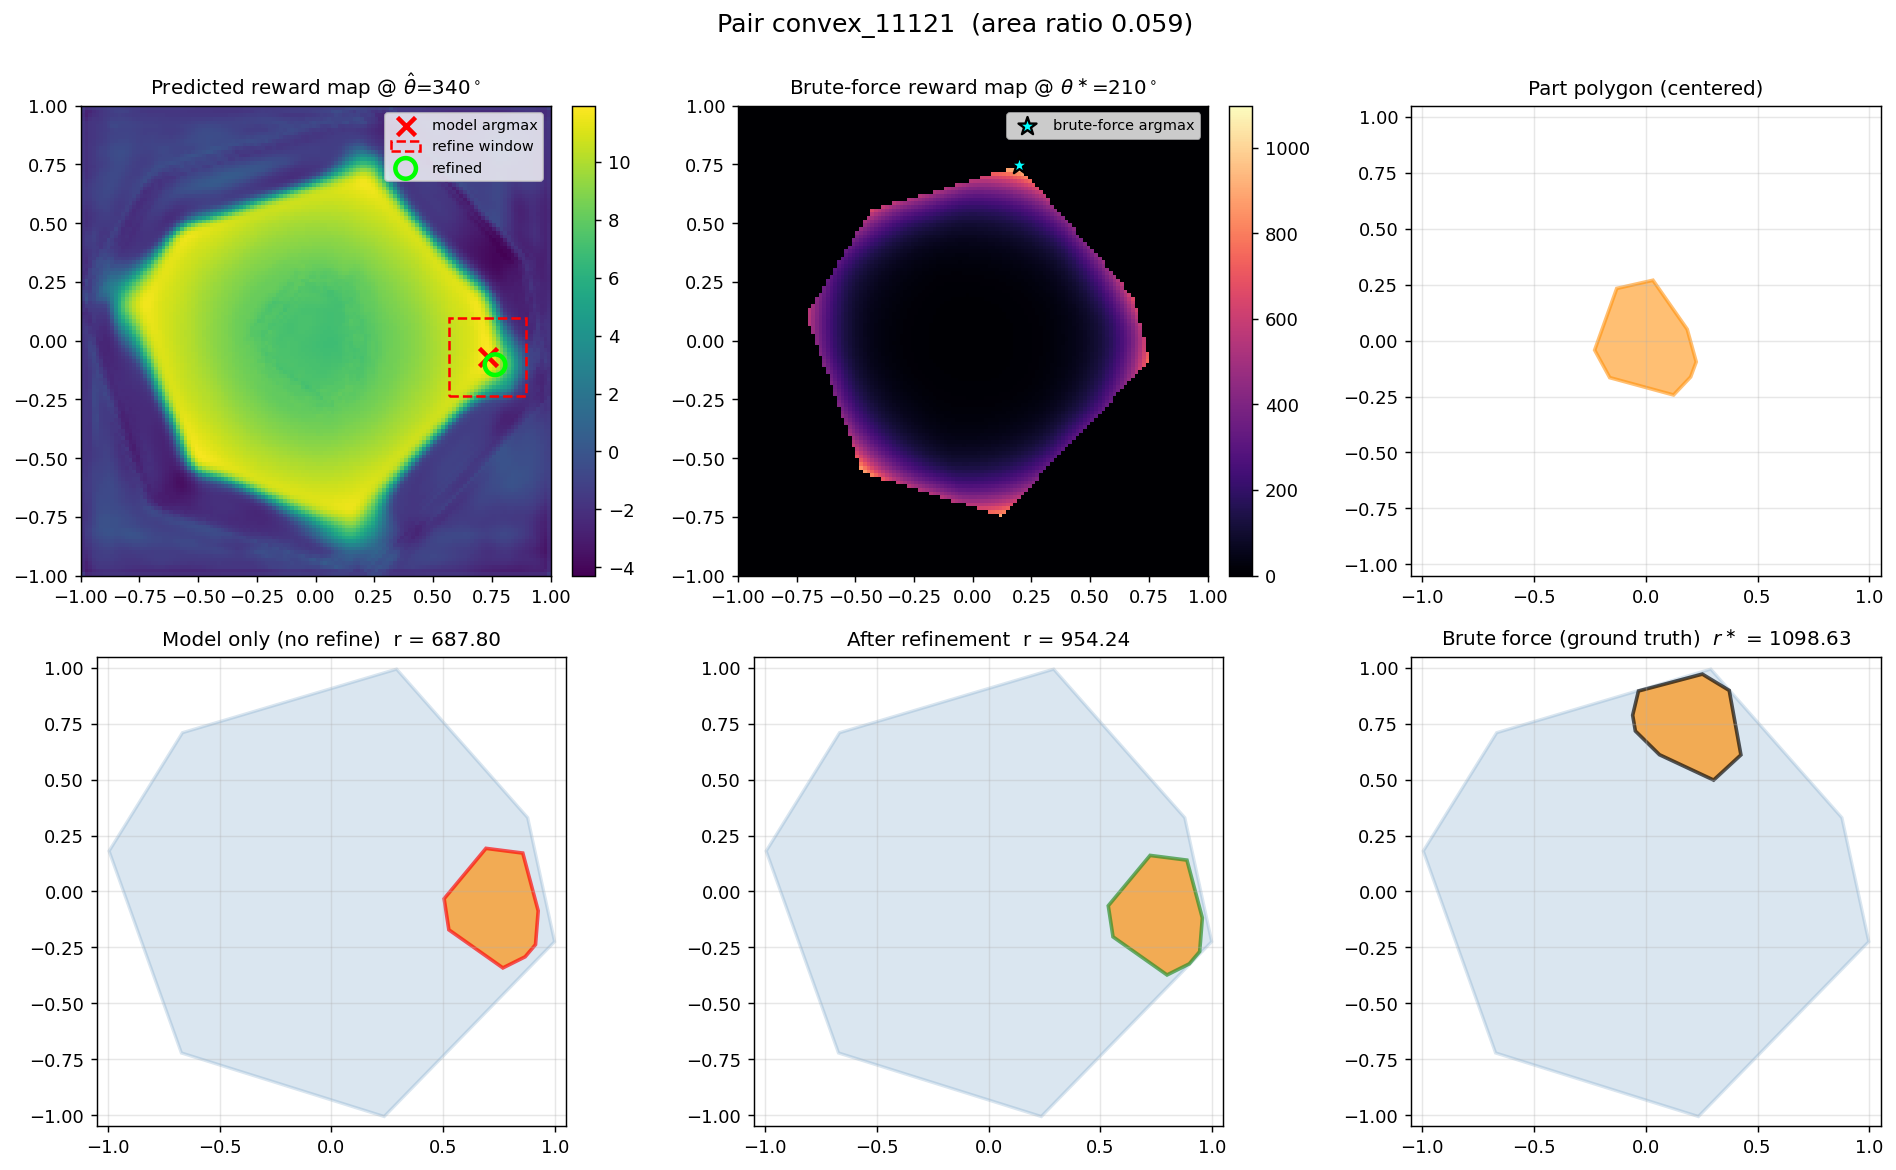
\includegraphics[width=\textwidth]{figs/convex_11121.png}
\end{figure}

\begin{center}\small
\begin{tabular}{lrrrr}
  \toprule
  Method & $\theta$ (deg) & $(x, y)$ & Reward & Recovery \\
  \midrule
  Brute force ($r^\ast$)    & 210 & $(+0.197, +0.748)$ & 1098.633 & 1.000 \\
  Model only                & 340 & $(+0.732, -0.071)$       & 687.801 & 0.626 \\
  Refined ($\pm10$\,px, $\pm2$\,$\theta$-bins) & 340 & $(+0.764, -0.102)$ & 954.235 & 0.869 \\
  \bottomrule
\end{tabular}
\end{center}

\begin{center}\small
\begin{tabular}{lr}
  \toprule
  Cost & Value \\
  \midrule
  Rasterize (36 rotated part masks)              & 4.7 ms \\
  Model forward (36 passes, batched)             & 45.6 ms \\
  Shapely refinement (2205 calls, target 2205)  & 771.5 ms \\
  \midrule
  Total                                          & 821.8 ms \\
  \bottomrule
\end{tabular}
\end{center}

\subsection{Pair convex\_11167 \quad\small\textmd{(area ratio 0.079)}}

\begin{figure}[H]
\centering
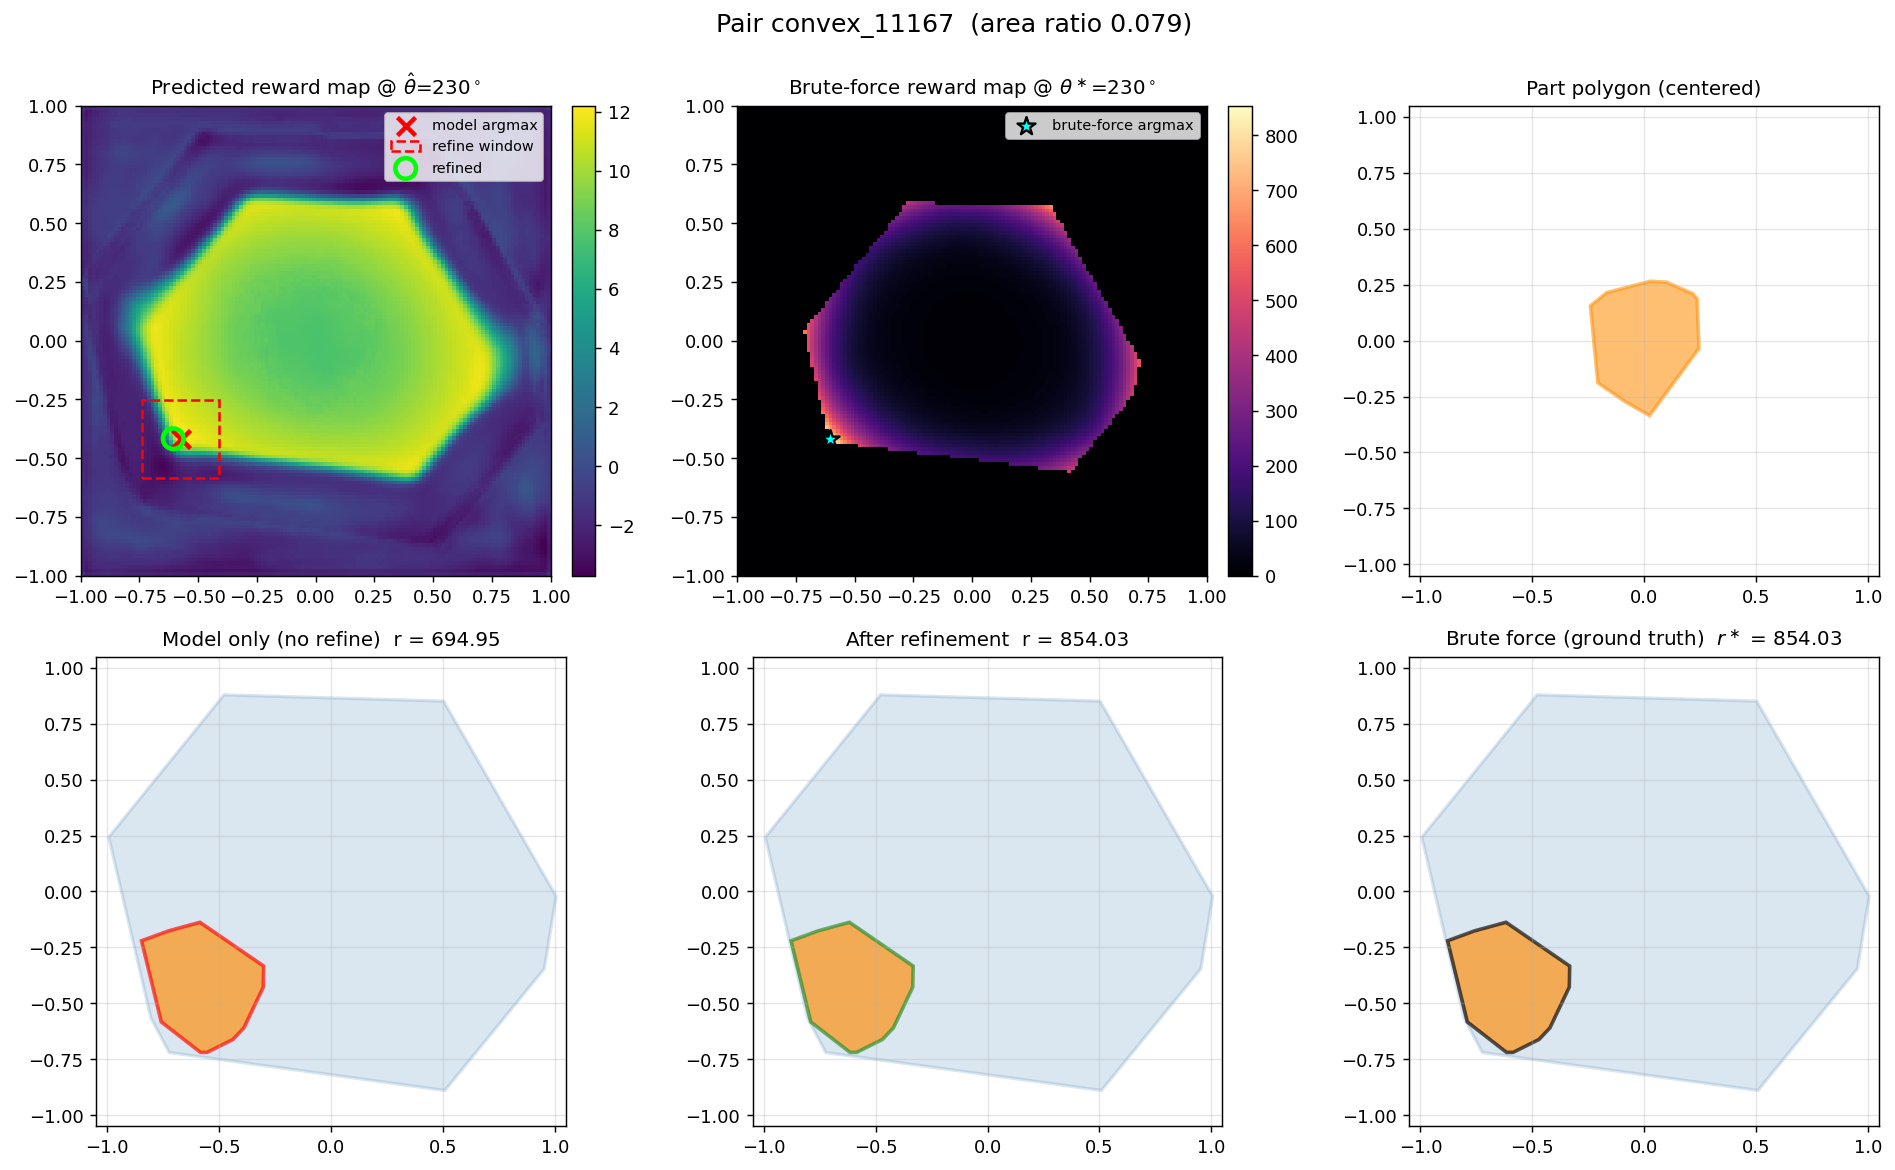
\includegraphics[width=\textwidth]{figs/convex_11167.png}
\end{figure}

\begin{center}\small
\begin{tabular}{lrrrr}
  \toprule
  Method & $\theta$ (deg) & $(x, y)$ & Reward & Recovery \\
  \midrule
  Brute force ($r^\ast$)    & 230 & $(-0.606, -0.417)$ & 854.025 & 1.000 \\
  Model only                & 230 & $(-0.575, -0.417)$       & 694.950 & 0.814 \\
  Refined ($\pm10$\,px, $\pm2$\,$\theta$-bins) & 230 & $(-0.606, -0.417)$ & 854.025 & 1.000 \\
  \bottomrule
\end{tabular}
\end{center}

\begin{center}\small
\begin{tabular}{lr}
  \toprule
  Cost & Value \\
  \midrule
  Rasterize (36 rotated part masks)              & 5.7 ms \\
  Model forward (36 passes, batched)             & 44.8 ms \\
  Shapely refinement (2205 calls, target 2205)  & 657.6 ms \\
  \midrule
  Total                                          & 708.1 ms \\
  \bottomrule
\end{tabular}
\end{center}

\subsection{Pair convex\_11408 \quad\small\textmd{(area ratio 0.542)}}

\begin{figure}[H]
\centering
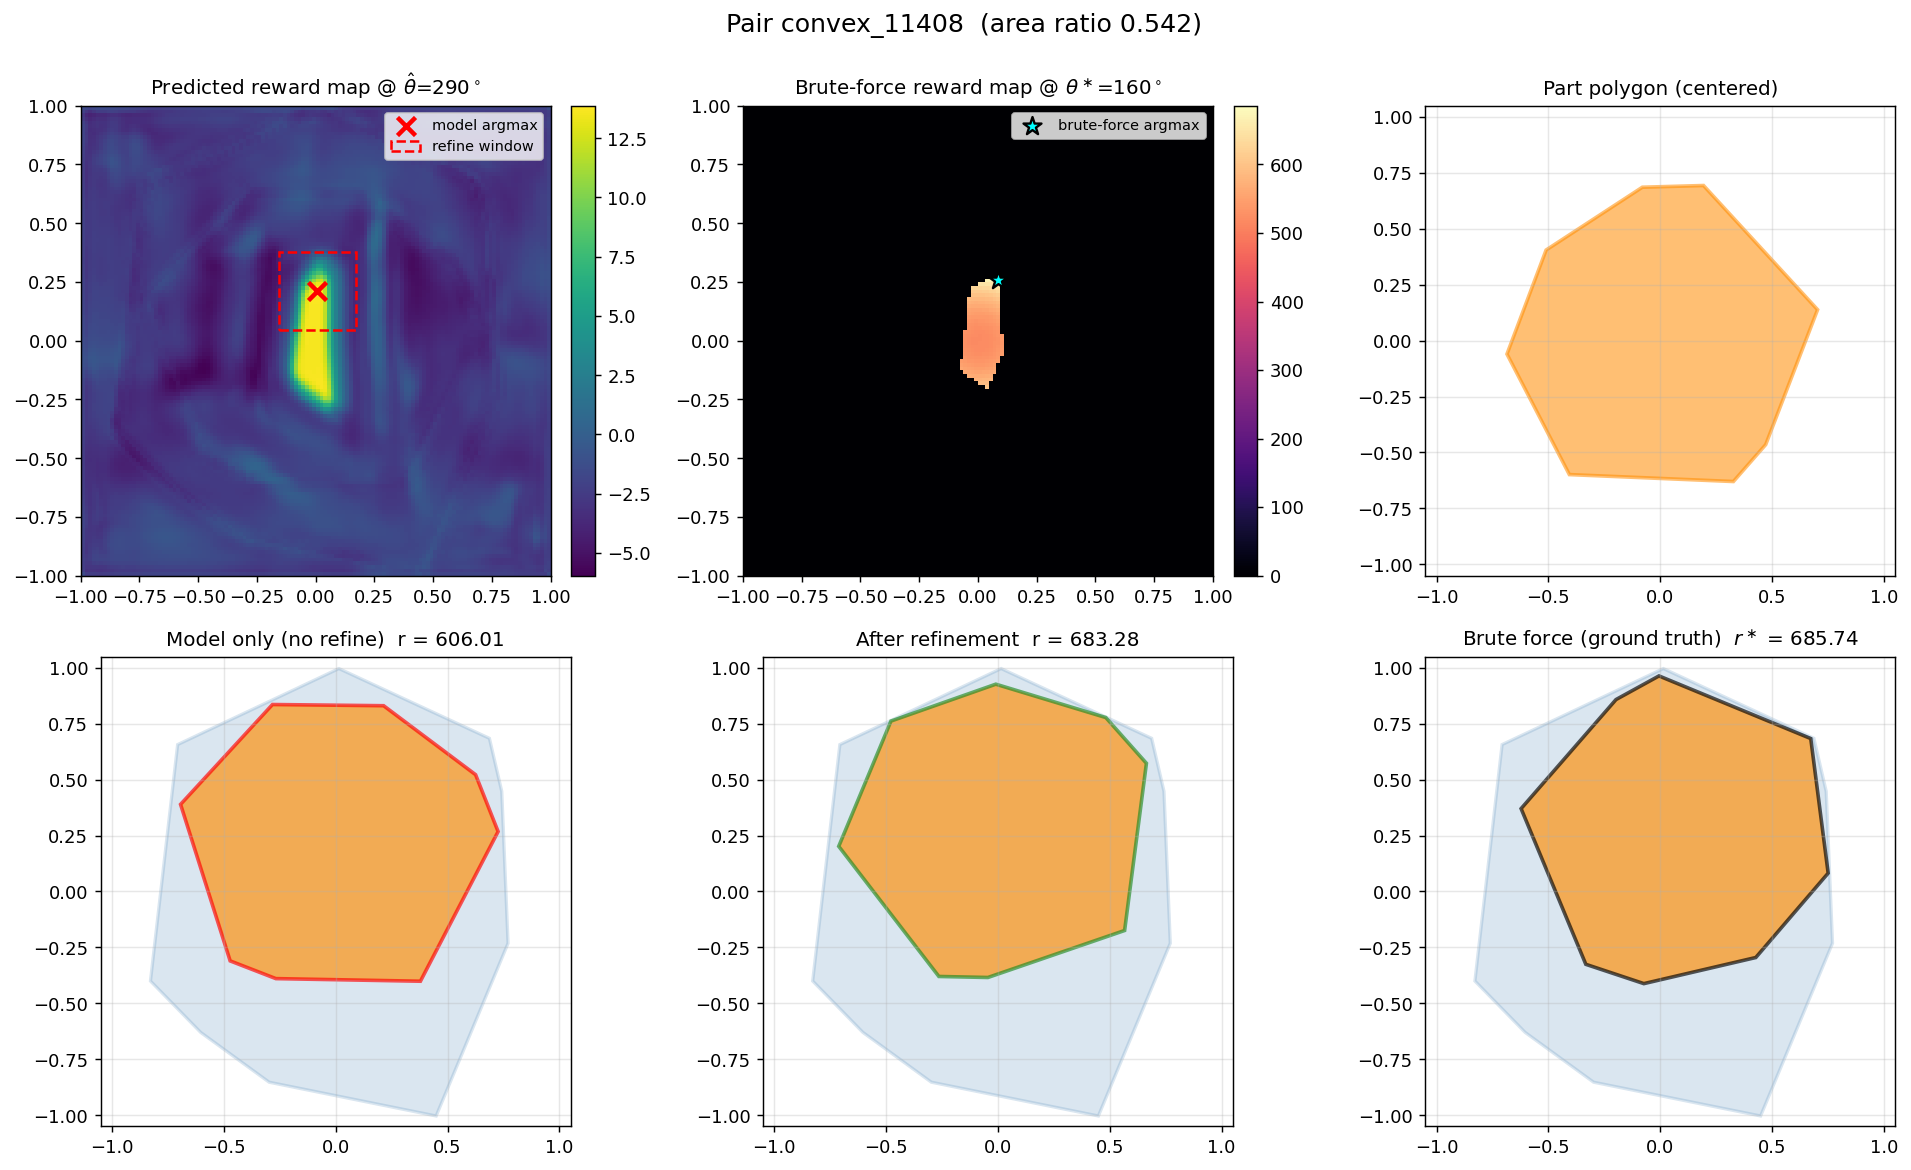
\includegraphics[width=\textwidth]{figs/convex_11408.png}
\end{figure}

\begin{center}\small
\begin{tabular}{lrrrr}
  \toprule
  Method & $\theta$ (deg) & $(x, y)$ & Reward & Recovery \\
  \midrule
  Brute force ($r^\ast$)    & 160 & $(+0.087, +0.260)$ & 685.735 & 1.000 \\
  Model only                & 290 & $(+0.008, +0.213)$       & 606.011 & 0.884 \\
  Refined ($\pm10$\,px, $\pm2$\,$\theta$-bins) & 310 & $(+0.008, +0.276)$ & 683.282 & 0.996 \\
  \bottomrule
\end{tabular}
\end{center}

\begin{center}\small
\begin{tabular}{lr}
  \toprule
  Cost & Value \\
  \midrule
  Rasterize (36 rotated part masks)              & 6.6 ms \\
  Model forward (36 passes, batched)             & 44.7 ms \\
  Shapely refinement (2205 calls, target 2205)  & 529.8 ms \\
  \midrule
  Total                                          & 581.1 ms \\
  \bottomrule
\end{tabular}
\end{center}

\subsection{Pair convex\_11557 \quad\small\textmd{(area ratio 0.338)}}

\begin{figure}[H]
\centering
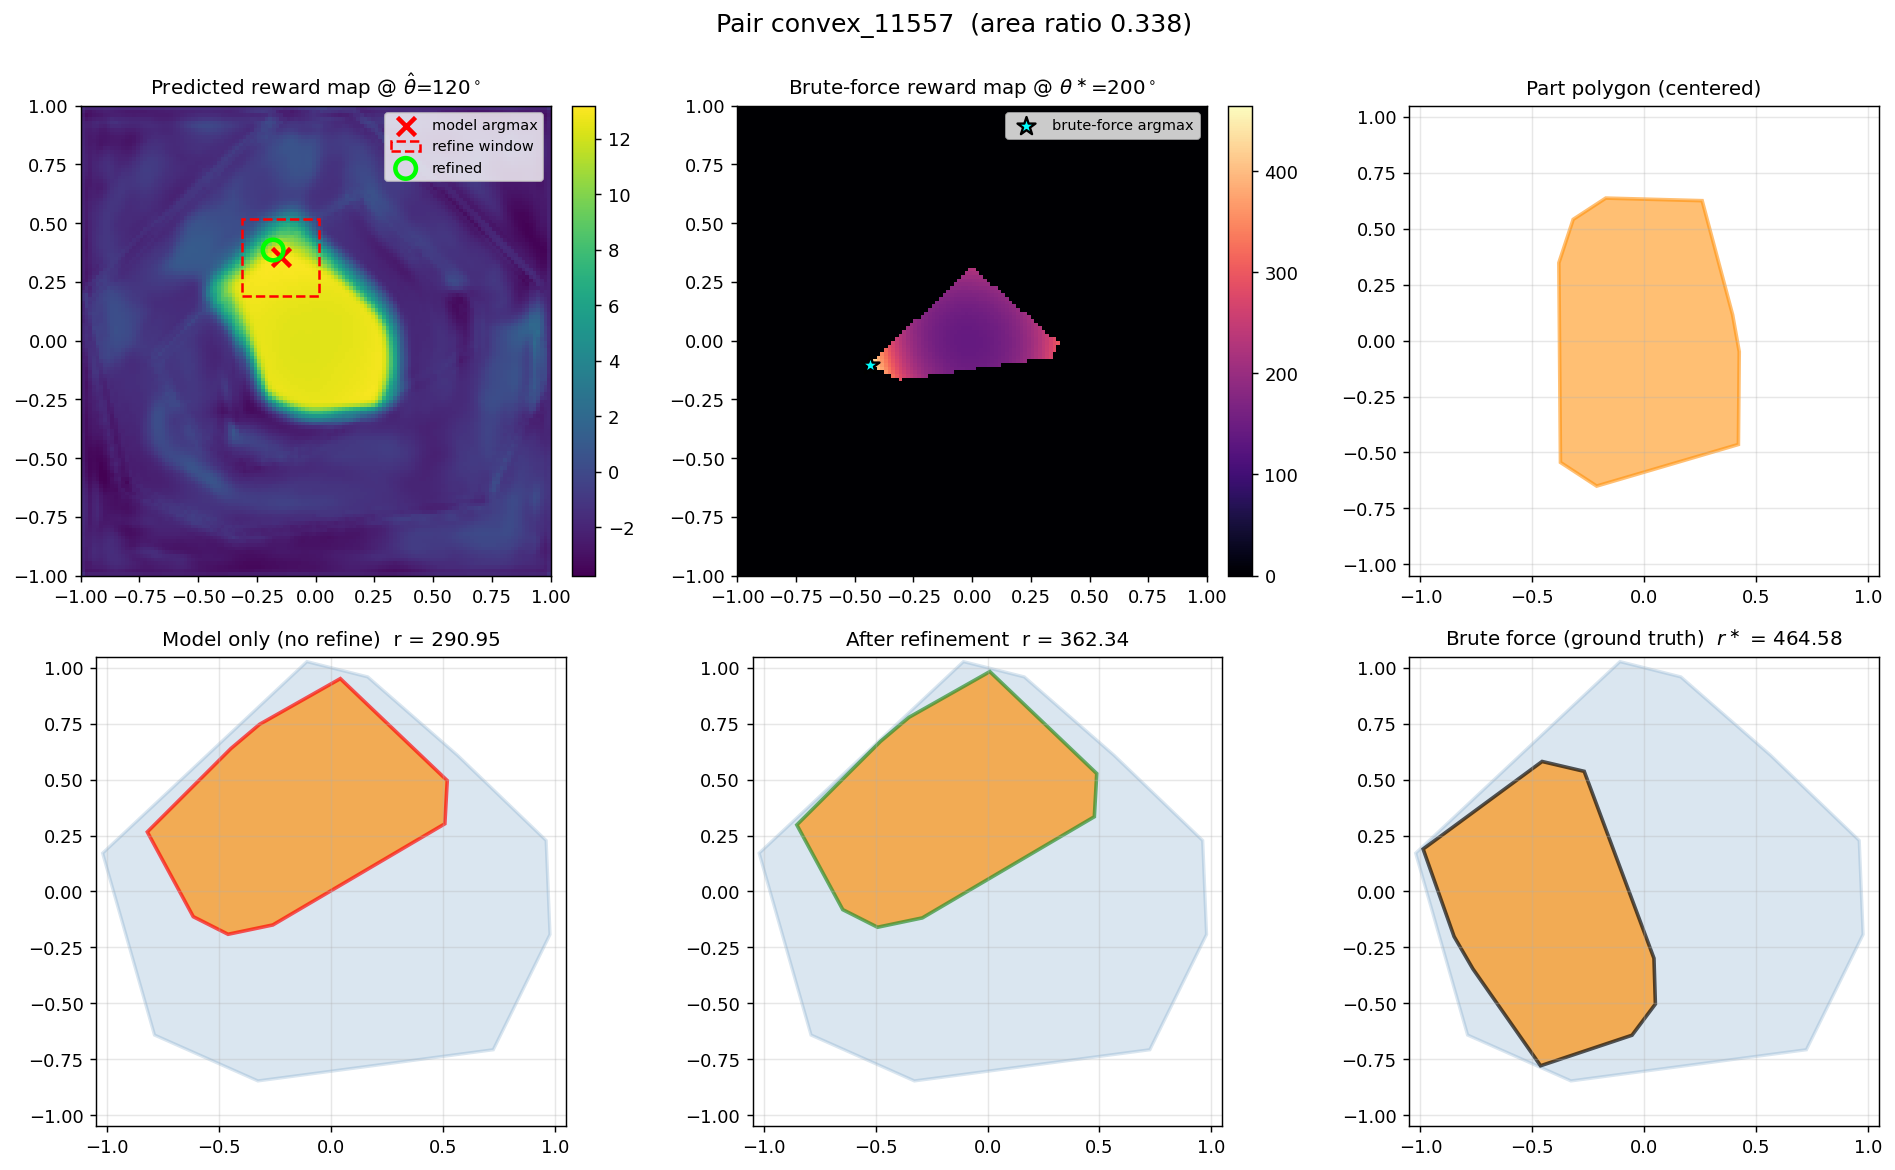
\includegraphics[width=\textwidth]{figs/convex_11557.png}
\end{figure}

\begin{center}\small
\begin{tabular}{lrrrr}
  \toprule
  Method & $\theta$ (deg) & $(x, y)$ & Reward & Recovery \\
  \midrule
  Brute force ($r^\ast$)    & 200 & $(-0.433, -0.102)$ & 464.579 & 1.000 \\
  Model only                & 120 & $(-0.150, +0.354)$       & 290.952 & 0.626 \\
  Refined ($\pm10$\,px, $\pm2$\,$\theta$-bins) & 120 & $(-0.181, +0.386)$ & 362.344 & 0.780 \\
  \bottomrule
\end{tabular}
\end{center}

\begin{center}\small
\begin{tabular}{lr}
  \toprule
  Cost & Value \\
  \midrule
  Rasterize (36 rotated part masks)              & 6.3 ms \\
  Model forward (36 passes, batched)             & 310.5 ms \\
  Shapely refinement (2205 calls, target 2205)  & 615.3 ms \\
  \midrule
  Total                                          & 932.1 ms \\
  \bottomrule
\end{tabular}
\end{center}

\subsection{Pair convex\_11578 \quad\small\textmd{(area ratio 0.575)}}

\begin{figure}[H]
\centering
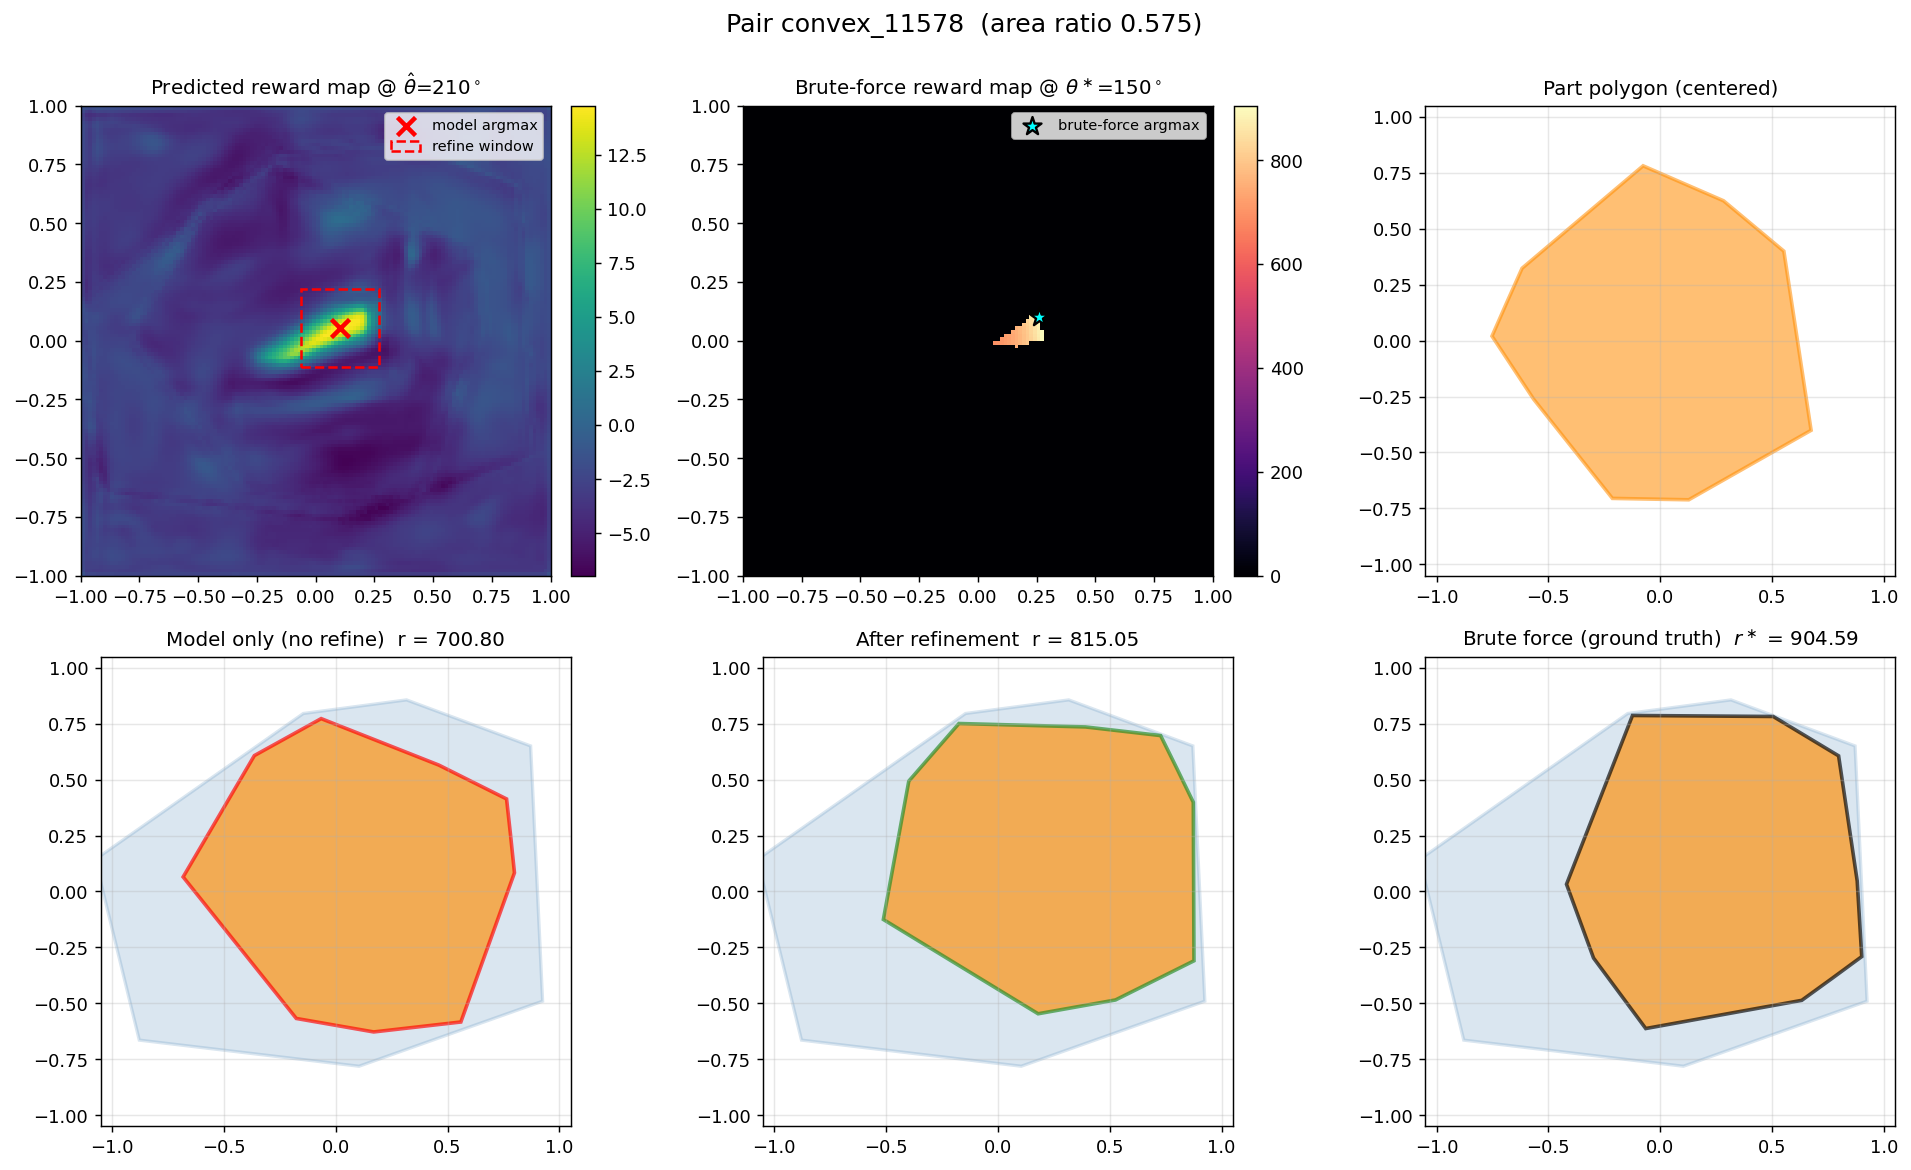
\includegraphics[width=\textwidth]{figs/convex_11578.png}
\end{figure}

\begin{center}\small
\begin{tabular}{lrrrr}
  \toprule
  Method & $\theta$ (deg) & $(x, y)$ & Reward & Recovery \\
  \midrule
  Brute force ($r^\ast$)    & 150 & $(+0.260, +0.102)$ & 904.592 & 1.000 \\
  Model only                & 210 & $(+0.102, +0.055)$       & 700.800 & 0.775 \\
  Refined ($\pm10$\,px, $\pm2$\,$\theta$-bins) & 230 & $(+0.228, +0.134)$ & 815.048 & 0.901 \\
  \bottomrule
\end{tabular}
\end{center}

\begin{center}\small
\begin{tabular}{lr}
  \toprule
  Cost & Value \\
  \midrule
  Rasterize (36 rotated part masks)              & 6.8 ms \\
  Model forward (36 passes, batched)             & 44.0 ms \\
  Shapely refinement (2205 calls, target 2205)  & 492.4 ms \\
  \midrule
  Total                                          & 543.2 ms \\
  \bottomrule
\end{tabular}
\end{center}

\subsection{Pair convex\_11774 \quad\small\textmd{(area ratio 0.390)}}

\begin{figure}[H]
\centering
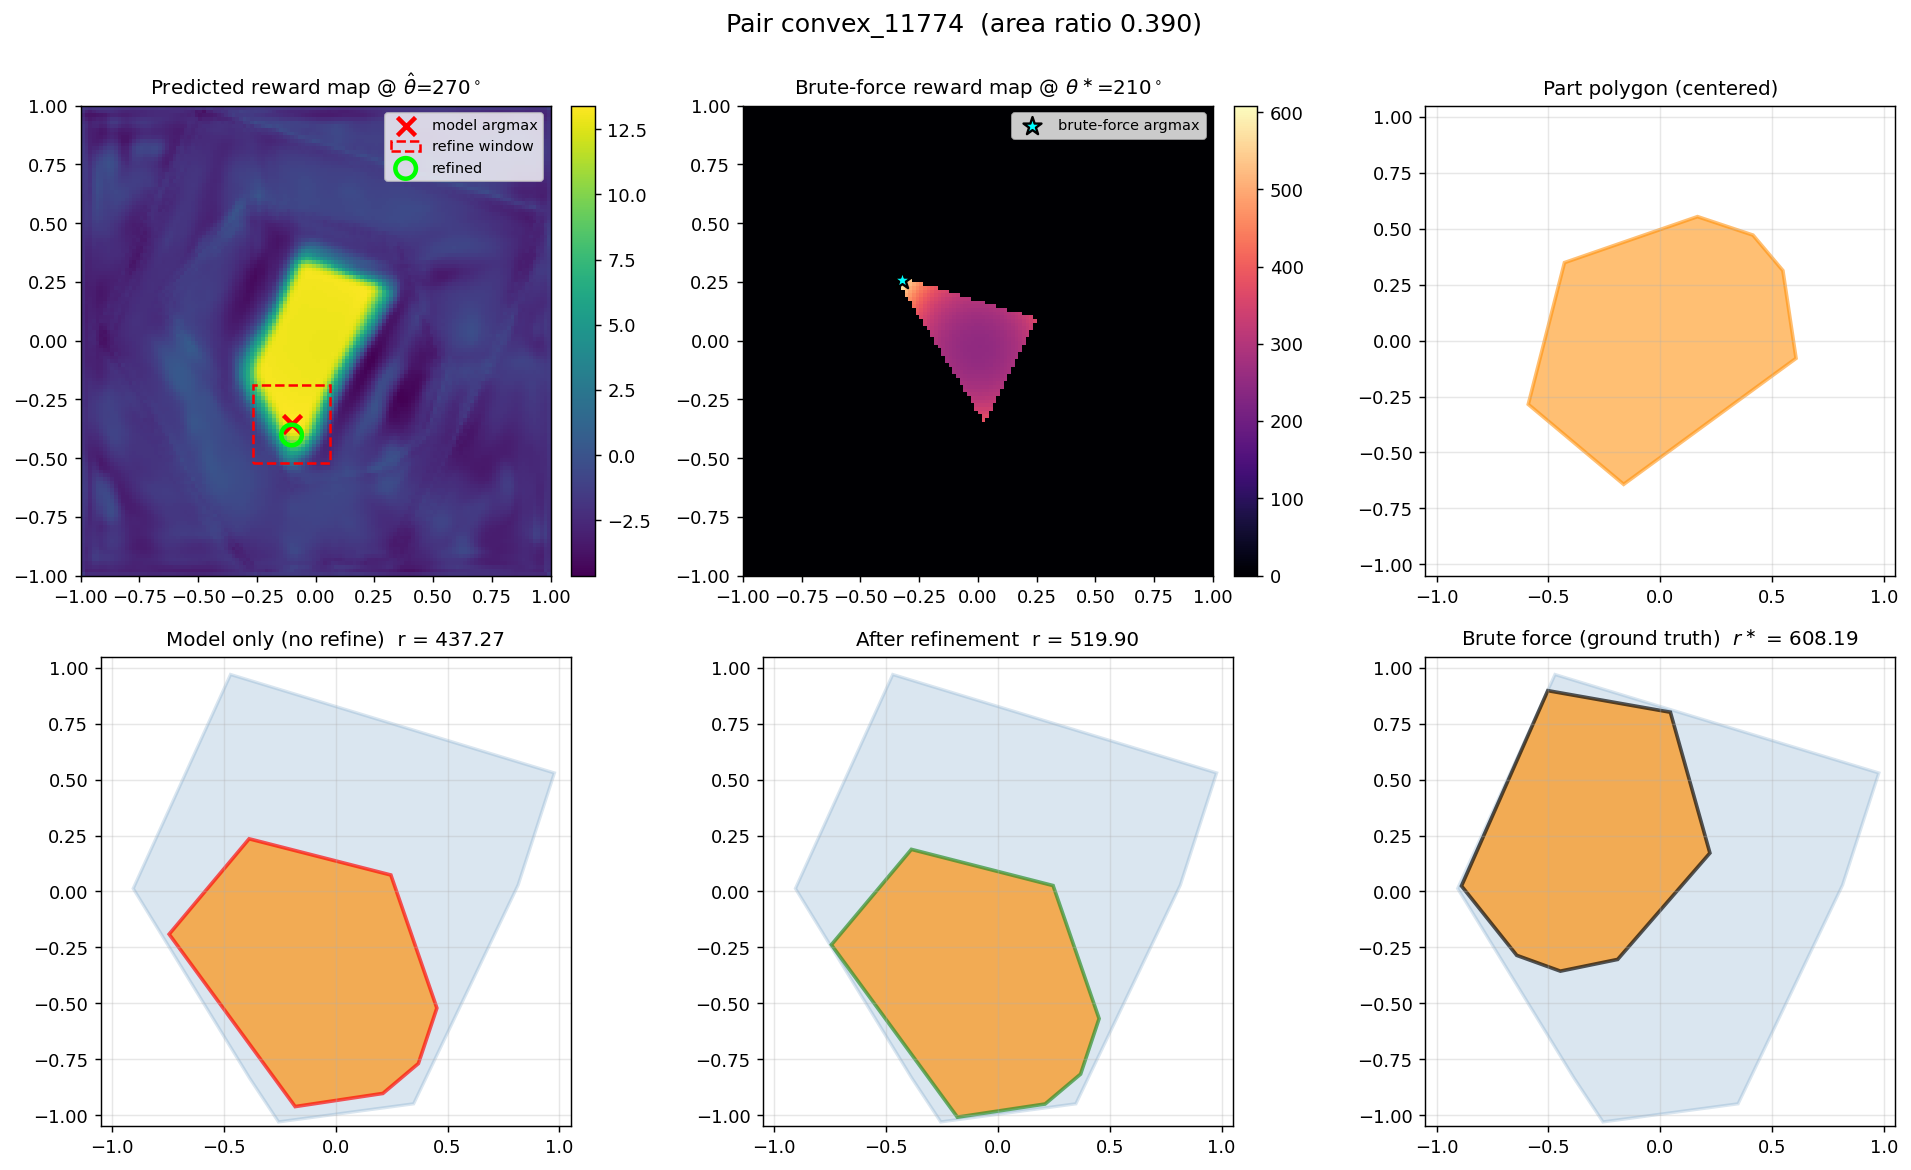
\includegraphics[width=\textwidth]{figs/convex_11774.png}
\end{figure}

\begin{center}\small
\begin{tabular}{lrrrr}
  \toprule
  Method & $\theta$ (deg) & $(x, y)$ & Reward & Recovery \\
  \midrule
  Brute force ($r^\ast$)    & 210 & $(-0.323, +0.260)$ & 608.192 & 1.000 \\
  Model only                & 270 & $(-0.102, -0.354)$       & 437.271 & 0.719 \\
  Refined ($\pm10$\,px, $\pm2$\,$\theta$-bins) & 270 & $(-0.102, -0.402)$ & 519.902 & 0.855 \\
  \bottomrule
\end{tabular}
\end{center}

\begin{center}\small
\begin{tabular}{lr}
  \toprule
  Cost & Value \\
  \midrule
  Rasterize (36 rotated part masks)              & 5.2 ms \\
  Model forward (36 passes, batched)             & 87.1 ms \\
  Shapely refinement (2205 calls, target 2205)  & 473.3 ms \\
  \midrule
  Total                                          & 565.6 ms \\
  \bottomrule
\end{tabular}
\end{center}

\subsection{Pair convex\_11811 \quad\small\textmd{(area ratio 0.519)}}

\begin{figure}[H]
\centering
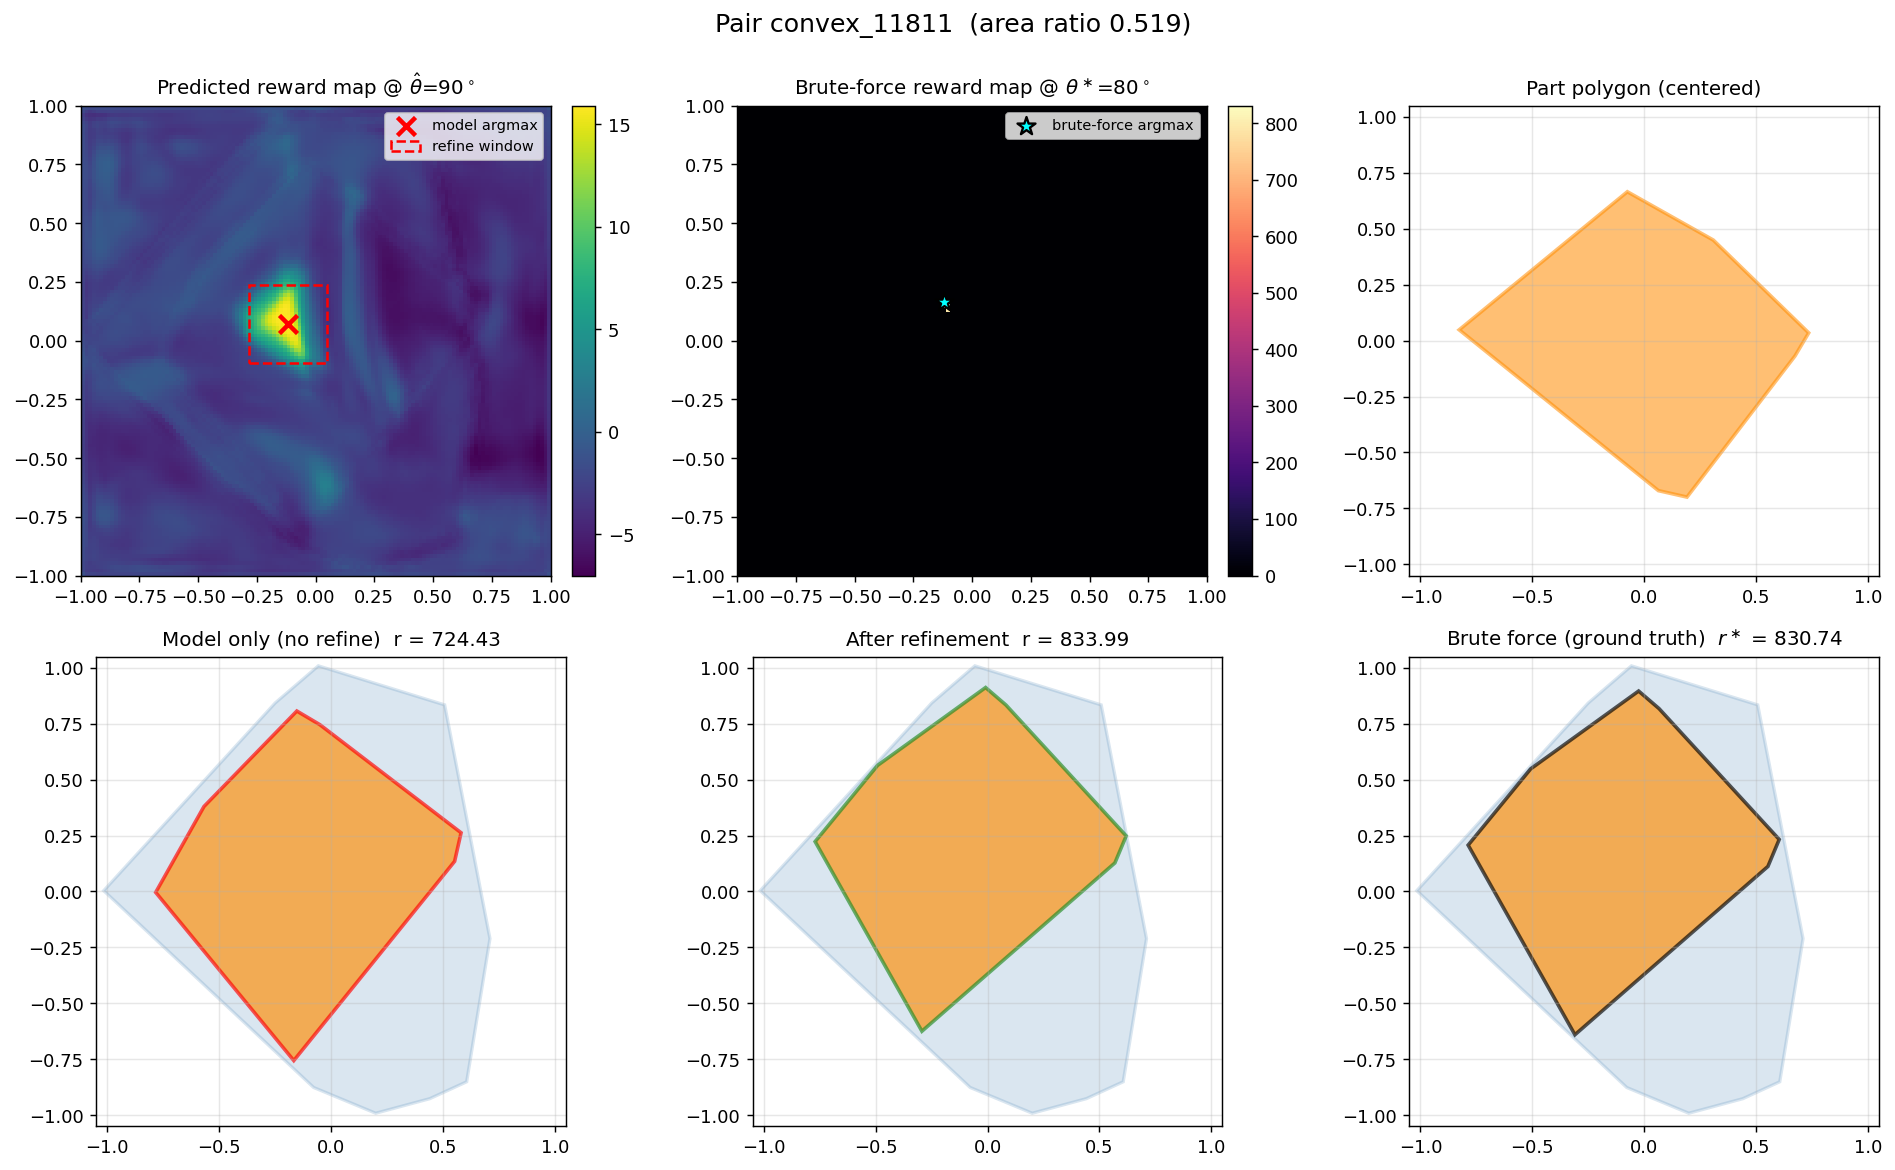
\includegraphics[width=\textwidth]{figs/convex_11811.png}
\end{figure}

\begin{center}\small
\begin{tabular}{lrrrr}
  \toprule
  Method & $\theta$ (deg) & $(x, y)$ & Reward & Recovery \\
  \midrule
  Brute force ($r^\ast$)    & 80 & $(-0.118, +0.165)$ & 830.735 & 1.000 \\
  Model only                & 90 & $(-0.118, +0.071)$       & 724.427 & 0.872 \\
  Refined ($\pm10$\,px, $\pm2$\,$\theta$-bins) & 80 & $(-0.102, +0.181)$ & 833.989 & 1.004 \\
  \bottomrule
\end{tabular}
\end{center}

\begin{center}\small
\begin{tabular}{lr}
  \toprule
  Cost & Value \\
  \midrule
  Rasterize (36 rotated part masks)              & 7.6 ms \\
  Model forward (36 passes, batched)             & 221.3 ms \\
  Shapely refinement (2205 calls, target 2205)  & 345.8 ms \\
  \midrule
  Total                                          & 574.7 ms \\
  \bottomrule
\end{tabular}
\end{center}

\subsection{Pair convex\_11895 \quad\small\textmd{(area ratio 0.131)}}

\begin{figure}[H]
\centering
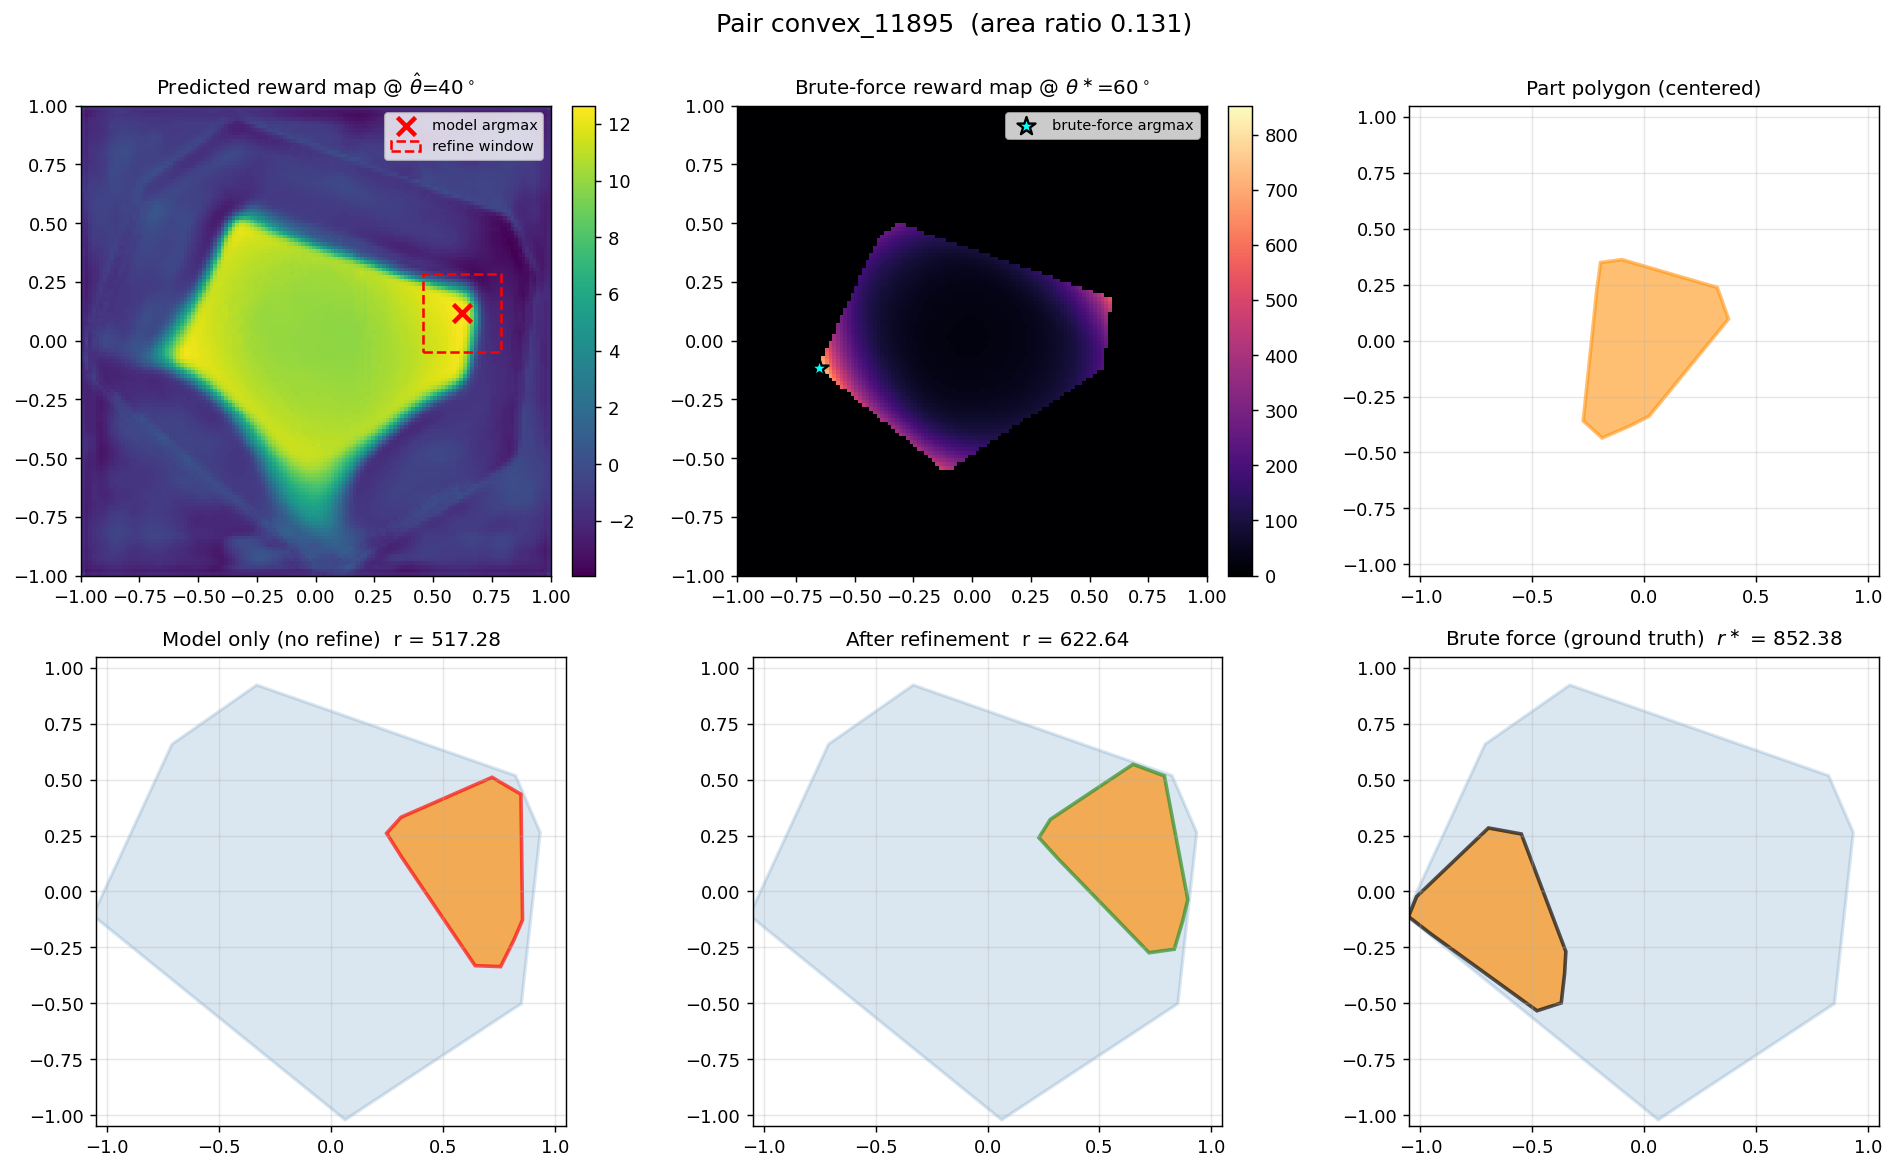
\includegraphics[width=\textwidth]{figs/convex_11895.png}
\end{figure}

\begin{center}\small
\begin{tabular}{lrrrr}
  \toprule
  Method & $\theta$ (deg) & $(x, y)$ & Reward & Recovery \\
  \midrule
  Brute force ($r^\ast$)    & 60 & $(-0.654, -0.118)$ & 852.383 & 1.000 \\
  Model only                & 40 & $(+0.622, +0.118)$       & 517.275 & 0.607 \\
  Refined ($\pm10$\,px, $\pm2$\,$\theta$-bins) & 50 & $(+0.622, +0.165)$ & 622.640 & 0.730 \\
  \bottomrule
\end{tabular}
\end{center}

\begin{center}\small
\begin{tabular}{lr}
  \toprule
  Cost & Value \\
  \midrule
  Rasterize (36 rotated part masks)              & 5.0 ms \\
  Model forward (36 passes, batched)             & 42.4 ms \\
  Shapely refinement (2205 calls, target 2205)  & 626.1 ms \\
  \midrule
  Total                                          & 673.6 ms \\
  \bottomrule
\end{tabular}
\end{center}

\newpage
\section{Examples --- Concave free-space pairs}
The free-space polygon is non-convex (random star polygon from \code{bo\_train\_pool\_10k.pkl}); the part remains convex.  The model and refinement use the same pipeline; brute-force $r^\ast$ is computed on the fly via \code{compute\_ifp\_exact} + exhaustive Shapely scoring inside the IFP (Section \ref{sec:inference}).  Same six-panel layout as before.

\subsection{Pair concave\_09002 \quad\small\textmd{(area ratio nan)}}

\begin{figure}[H]
\centering
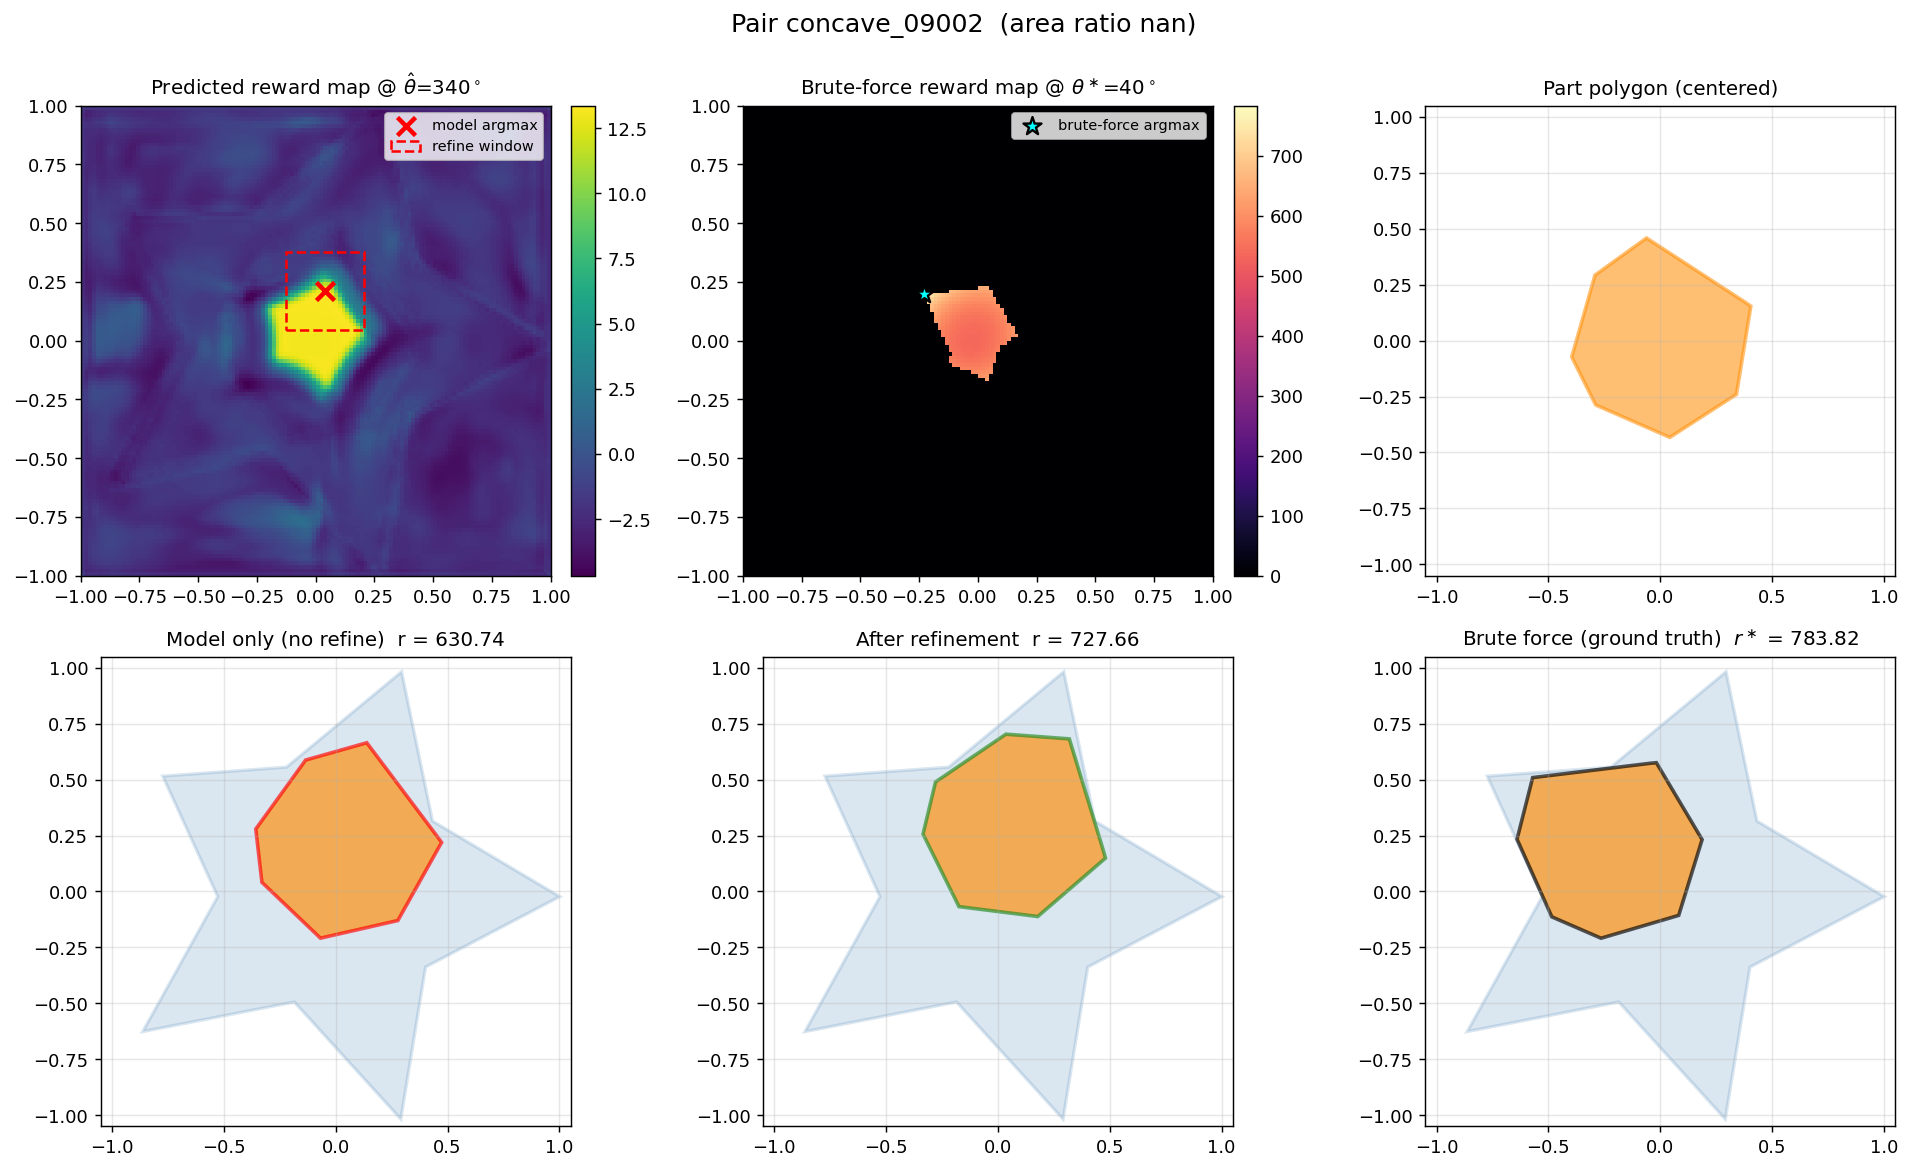
\includegraphics[width=\textwidth]{figs/concave_09002.png}
\end{figure}

\begin{center}\small
\begin{tabular}{lrrrr}
  \toprule
  Method & $\theta$ (deg) & $(x, y)$ & Reward & Recovery \\
  \midrule
  Brute force ($r^\ast$)    & 40 & $(-0.228, +0.197)$ & 783.819 & 1.000 \\
  Model only                & 340 & $(+0.039, +0.213)$       & 630.739 & 0.805 \\
  Refined ($\pm10$\,px, $\pm2$\,$\theta$-bins) & 320 & $(+0.071, +0.291)$ & 727.659 & 0.928 \\
  \bottomrule
\end{tabular}
\end{center}

\begin{center}\small
\begin{tabular}{lr}
  \toprule
  Cost & Value \\
  \midrule
  Rasterize (36 rotated part masks)              & 6.1 ms \\
  Model forward (36 passes, batched)             & 281.6 ms \\
  Shapely refinement (2205 calls, target 2205)  & 631.7 ms \\
  \midrule
  Total                                          & 919.4 ms \\
  \bottomrule
\end{tabular}
\end{center}

\subsection{Pair concave\_09033 \quad\small\textmd{(area ratio nan)}}

\begin{figure}[H]
\centering
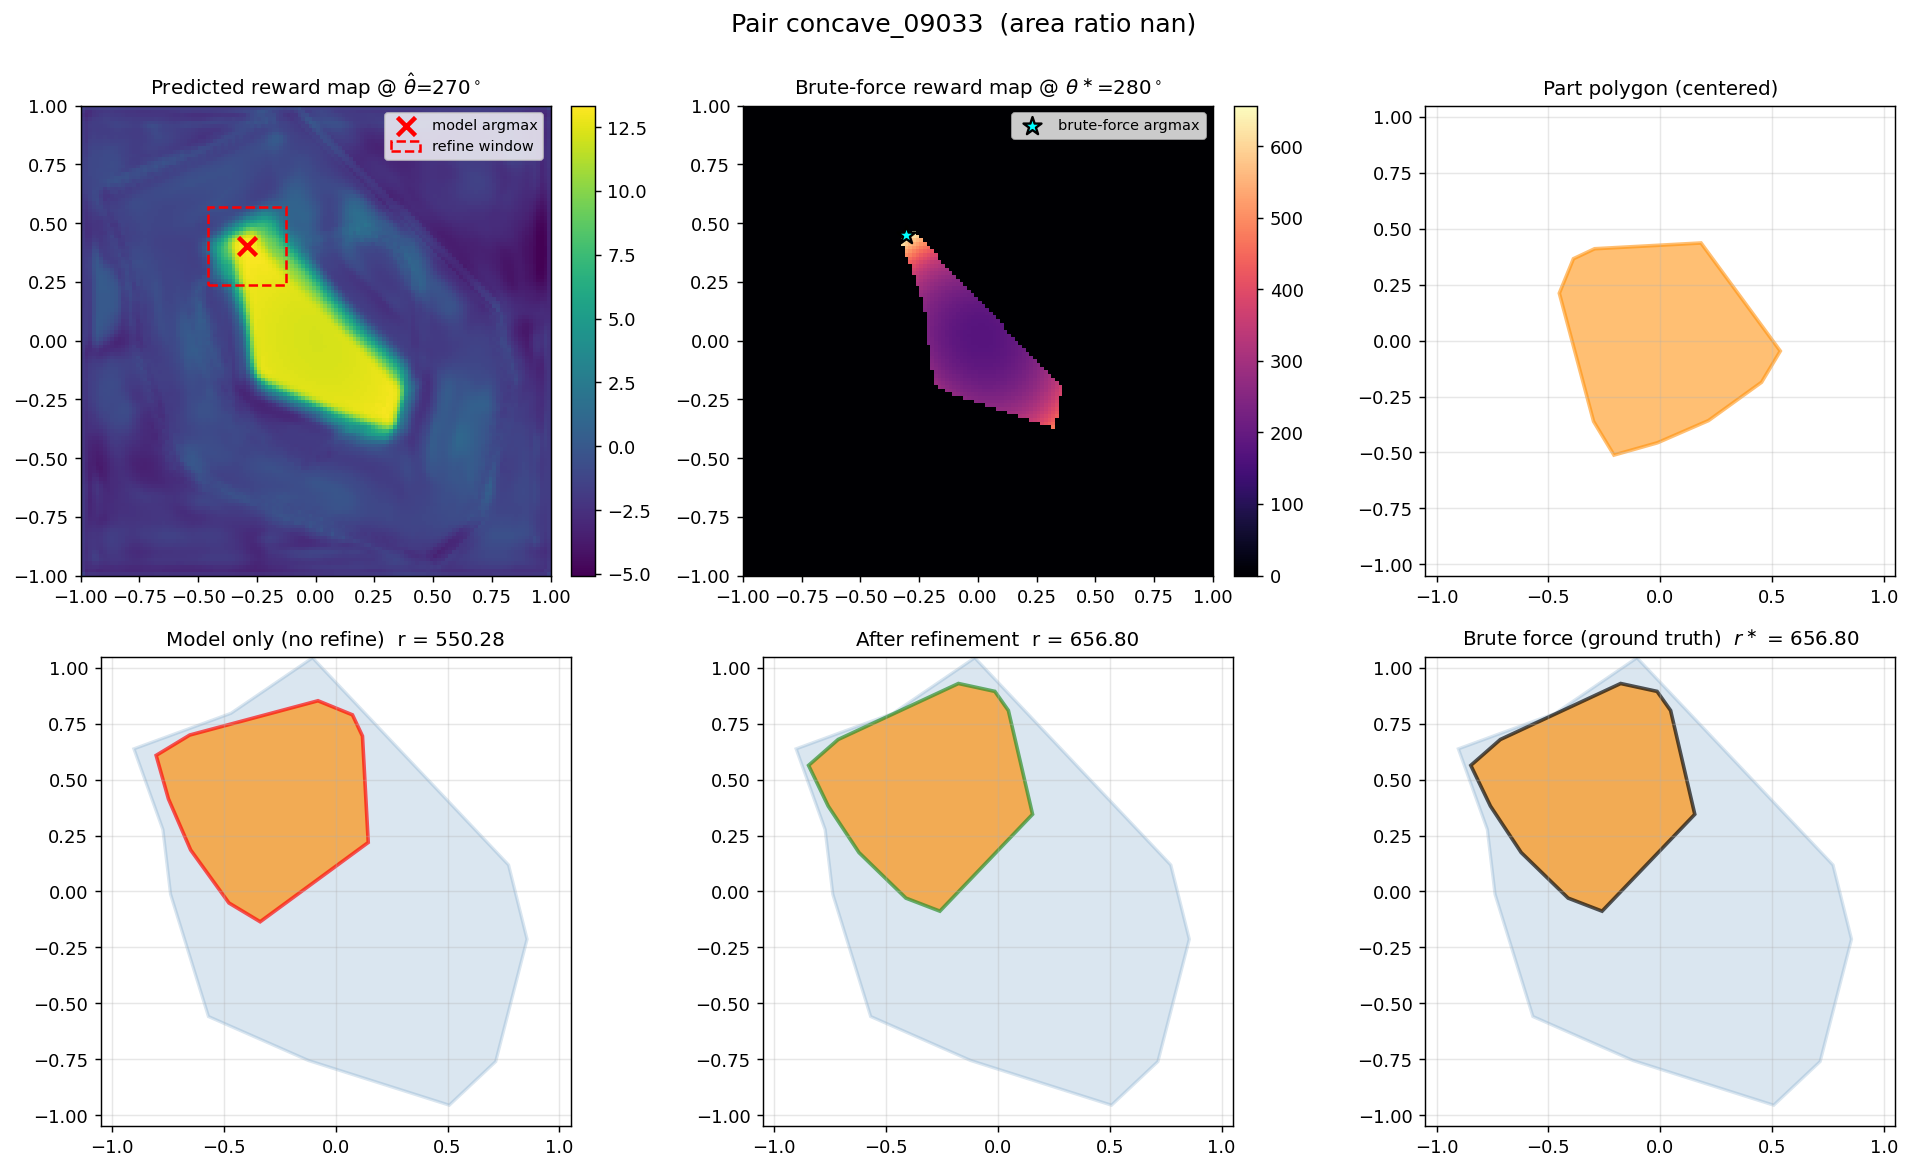
\includegraphics[width=\textwidth]{figs/concave_09033.png}
\end{figure}

\begin{center}\small
\begin{tabular}{lrrrr}
  \toprule
  Method & $\theta$ (deg) & $(x, y)$ & Reward & Recovery \\
  \midrule
  Brute force ($r^\ast$)    & 280 & $(-0.307, +0.449)$ & 656.799 & 1.000 \\
  Model only                & 270 & $(-0.291, +0.402)$       & 550.279 & 0.838 \\
  Refined ($\pm10$\,px, $\pm2$\,$\theta$-bins) & 280 & $(-0.307, +0.449)$ & 656.798 & 1.000 \\
  \bottomrule
\end{tabular}
\end{center}

\begin{center}\small
\begin{tabular}{lr}
  \toprule
  Cost & Value \\
  \midrule
  Rasterize (36 rotated part masks)              & 5.2 ms \\
  Model forward (36 passes, batched)             & 404.5 ms \\
  Shapely refinement (2205 calls, target 2205)  & 504.6 ms \\
  \midrule
  Total                                          & 914.4 ms \\
  \bottomrule
\end{tabular}
\end{center}

\subsection{Pair concave\_09392 \quad\small\textmd{(area ratio nan)}}

\begin{figure}[H]
\centering
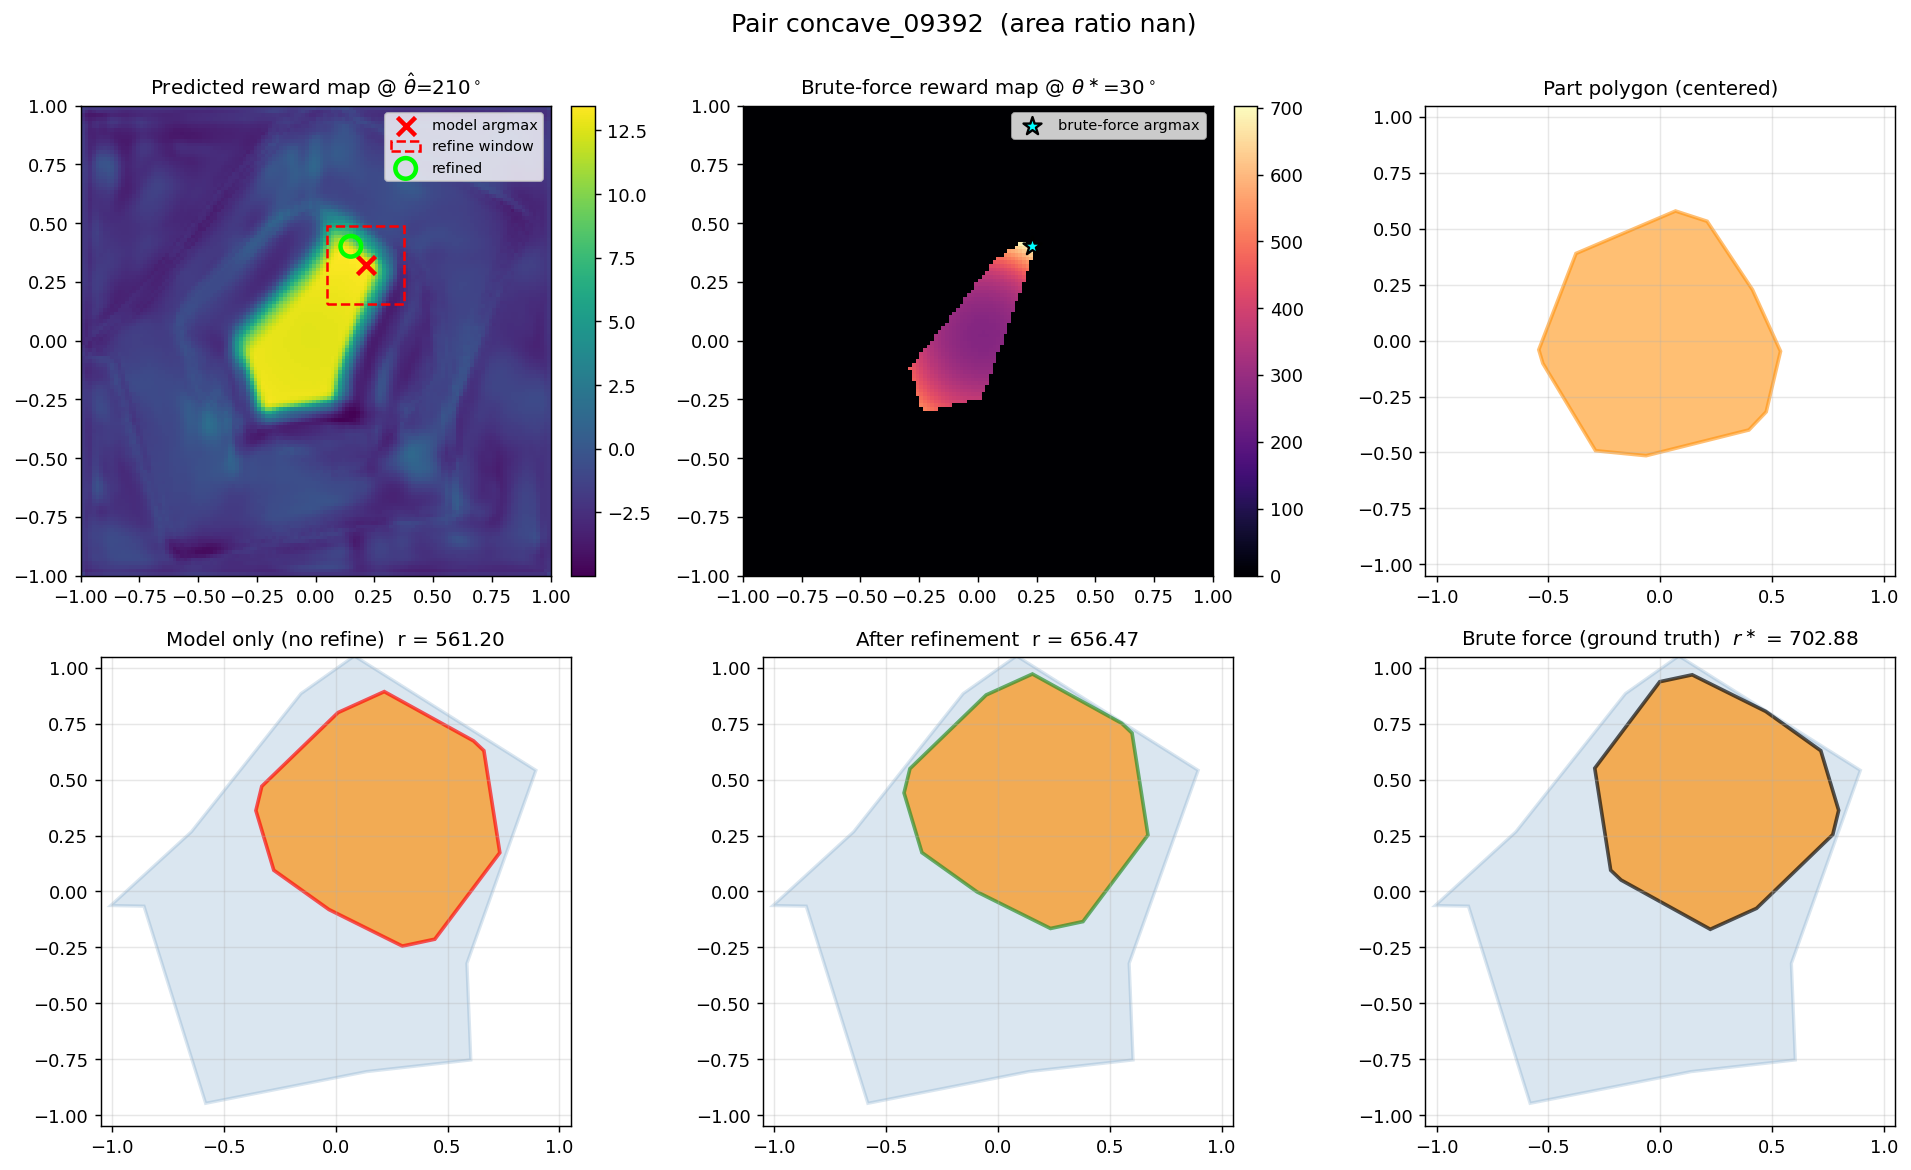
\includegraphics[width=\textwidth]{figs/concave_09392.png}
\end{figure}

\begin{center}\small
\begin{tabular}{lrrrr}
  \toprule
  Method & $\theta$ (deg) & $(x, y)$ & Reward & Recovery \\
  \midrule
  Brute force ($r^\ast$)    & 30 & $(+0.228, +0.402)$ & 702.877 & 1.000 \\
  Model only                & 210 & $(+0.213, +0.323)$       & 561.201 & 0.798 \\
  Refined ($\pm10$\,px, $\pm2$\,$\theta$-bins) & 210 & $(+0.150, +0.402)$ & 656.467 & 0.934 \\
  \bottomrule
\end{tabular}
\end{center}

\begin{center}\small
\begin{tabular}{lr}
  \toprule
  Cost & Value \\
  \midrule
  Rasterize (36 rotated part masks)              & 6.7 ms \\
  Model forward (36 passes, batched)             & 432.1 ms \\
  Shapely refinement (2205 calls, target 2205)  & 626.4 ms \\
  \midrule
  Total                                          & 1065.2 ms \\
  \bottomrule
\end{tabular}
\end{center}

\subsection{Pair concave\_09553 \quad\small\textmd{(area ratio nan)}}

\begin{figure}[H]
\centering
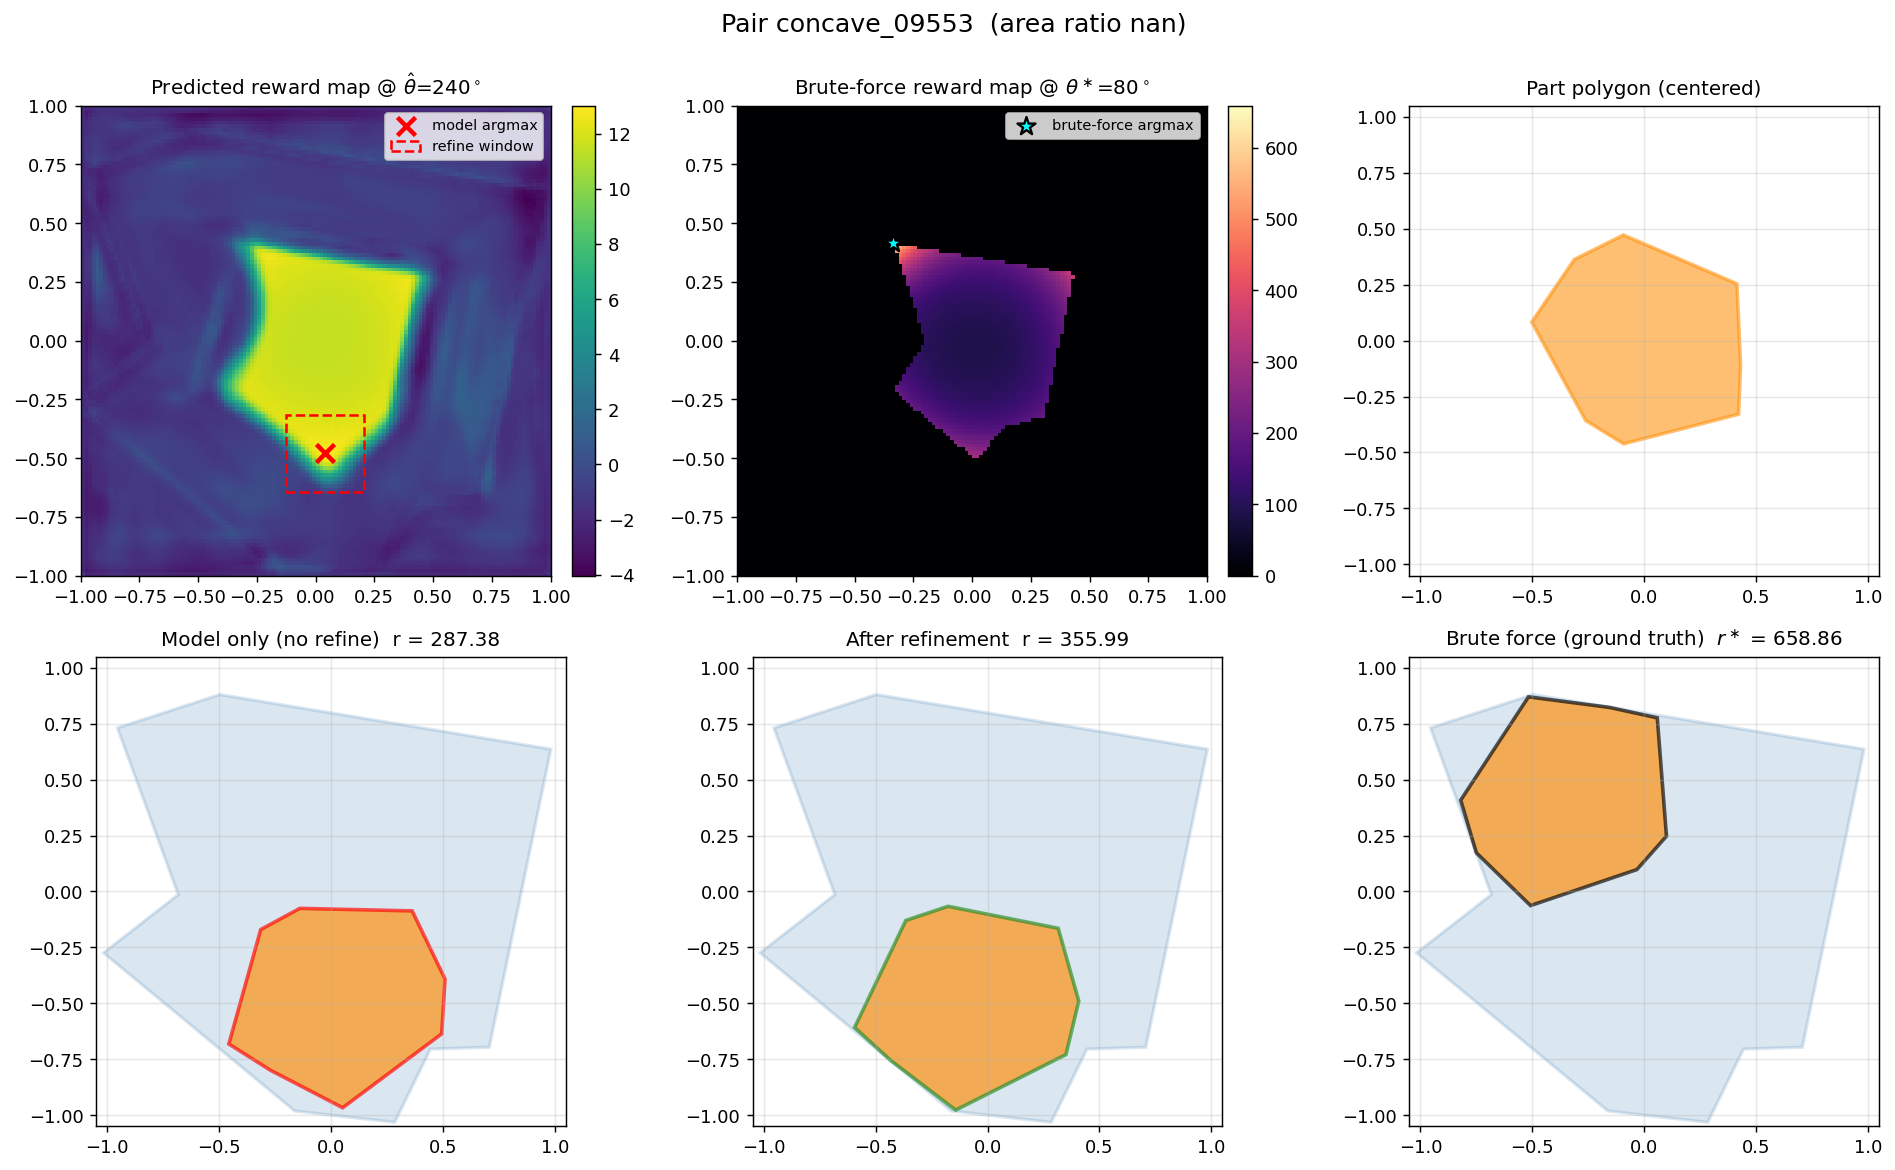
\includegraphics[width=\textwidth]{figs/concave_09553.png}
\end{figure}

\begin{center}\small
\begin{tabular}{lrrrr}
  \toprule
  Method & $\theta$ (deg) & $(x, y)$ & Reward & Recovery \\
  \midrule
  Brute force ($r^\ast$)    & 80 & $(-0.339, +0.417)$ & 658.856 & 1.000 \\
  Model only                & 240 & $(+0.039, -0.480)$       & 287.381 & 0.436 \\
  Refined ($\pm10$\,px, $\pm2$\,$\theta$-bins) & 230 & $(-0.071, -0.496)$ & 355.985 & 0.540 \\
  \bottomrule
\end{tabular}
\end{center}

\begin{center}\small
\begin{tabular}{lr}
  \toprule
  Cost & Value \\
  \midrule
  Rasterize (36 rotated part masks)              & 5.2 ms \\
  Model forward (36 passes, batched)             & 265.8 ms \\
  Shapely refinement (2205 calls, target 2205)  & 649.8 ms \\
  \midrule
  Total                                          & 920.8 ms \\
  \bottomrule
\end{tabular}
\end{center}

\subsection{Pair concave\_09764 \quad\small\textmd{(area ratio nan)}}

\begin{figure}[H]
\centering
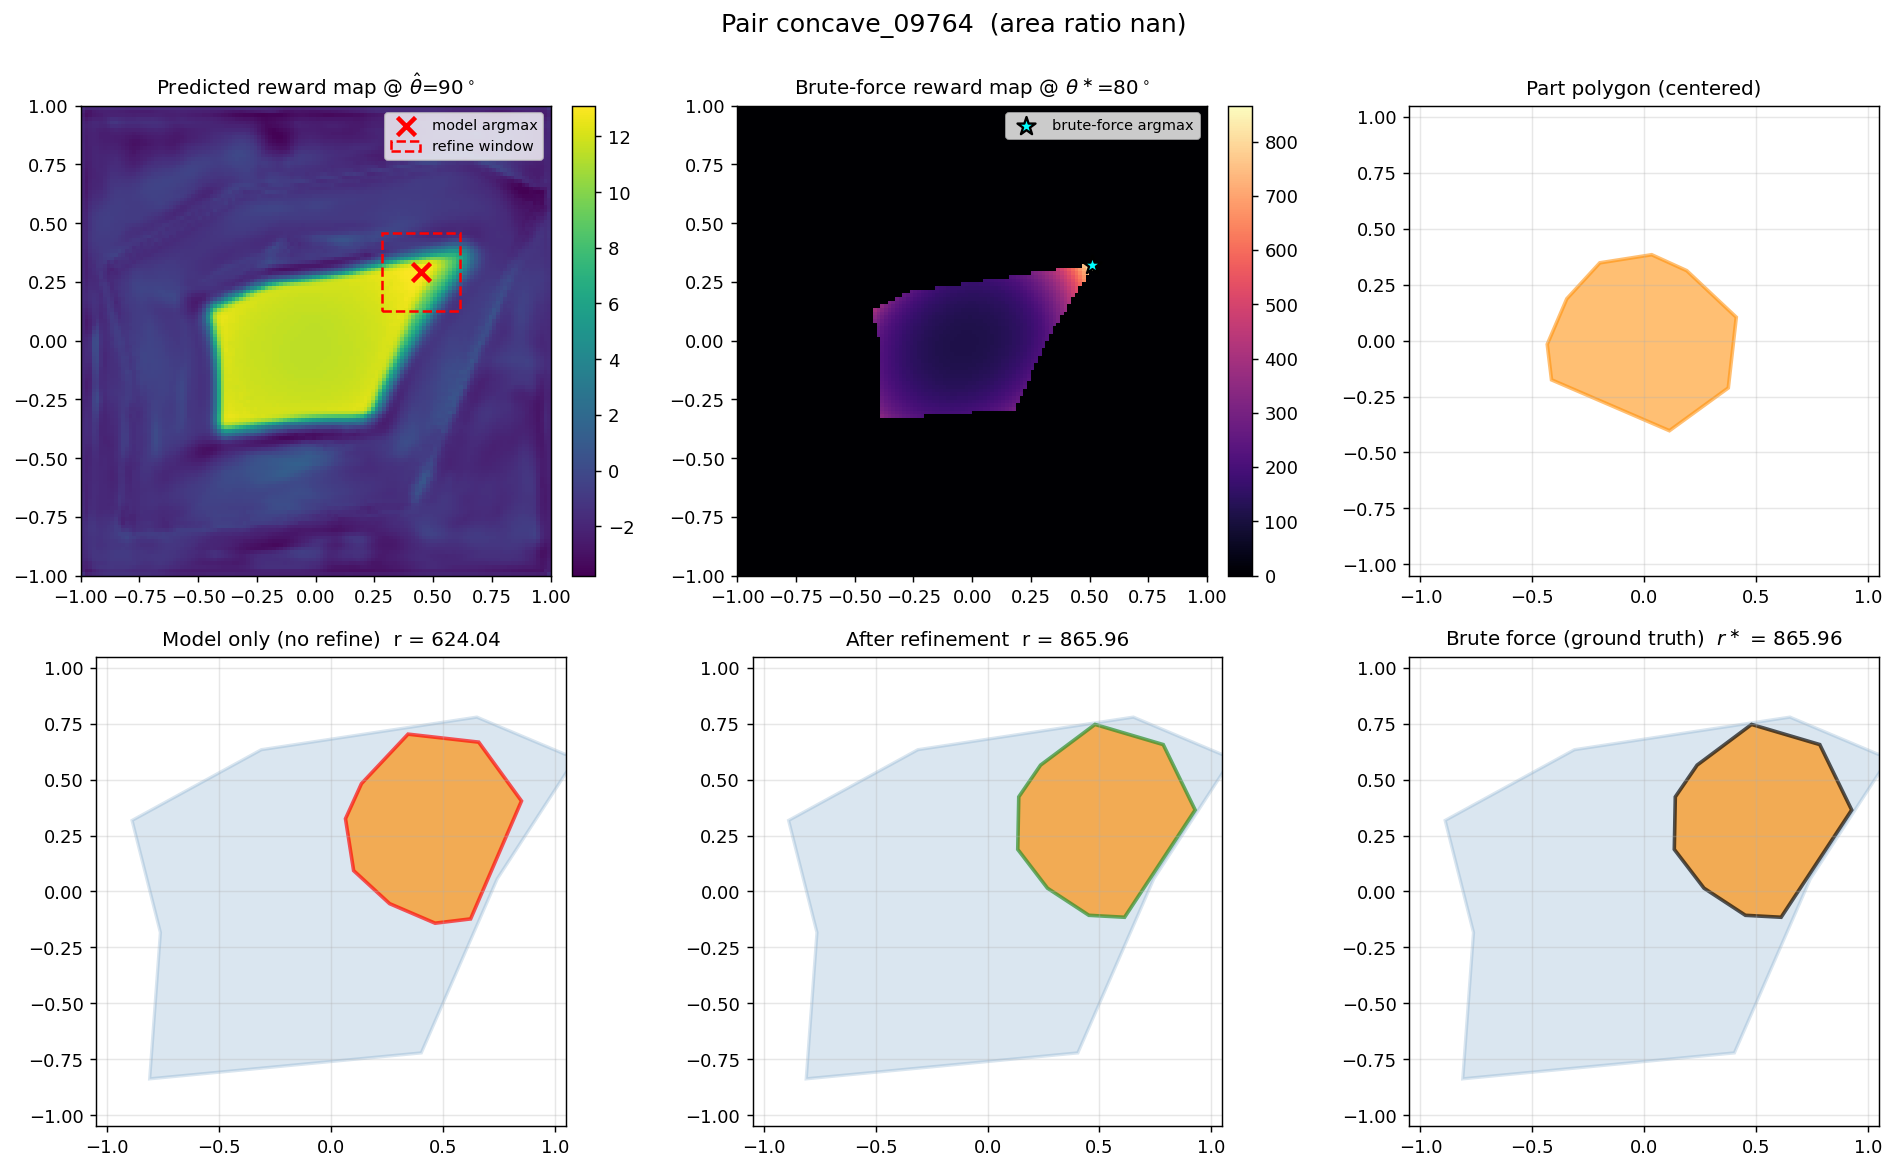
\includegraphics[width=\textwidth]{figs/concave_09764.png}
\end{figure}

\begin{center}\small
\begin{tabular}{lrrrr}
  \toprule
  Method & $\theta$ (deg) & $(x, y)$ & Reward & Recovery \\
  \midrule
  Brute force ($r^\ast$)    & 80 & $(+0.512, +0.323)$ & 865.964 & 1.000 \\
  Model only                & 90 & $(+0.449, +0.291)$       & 624.041 & 0.721 \\
  Refined ($\pm10$\,px, $\pm2$\,$\theta$-bins) & 80 & $(+0.512, +0.323)$ & 865.964 & 1.000 \\
  \bottomrule
\end{tabular}
\end{center}

\begin{center}\small
\begin{tabular}{lr}
  \toprule
  Cost & Value \\
  \midrule
  Rasterize (36 rotated part masks)              & 8.7 ms \\
  Model forward (36 passes, batched)             & 348.8 ms \\
  Shapely refinement (2205 calls, target 2205)  & 498.5 ms \\
  \midrule
  Total                                          & 856.0 ms \\
  \bottomrule
\end{tabular}
\end{center}

\subsection{Pair concave\_09854 \quad\small\textmd{(area ratio nan)}}

\begin{figure}[H]
\centering
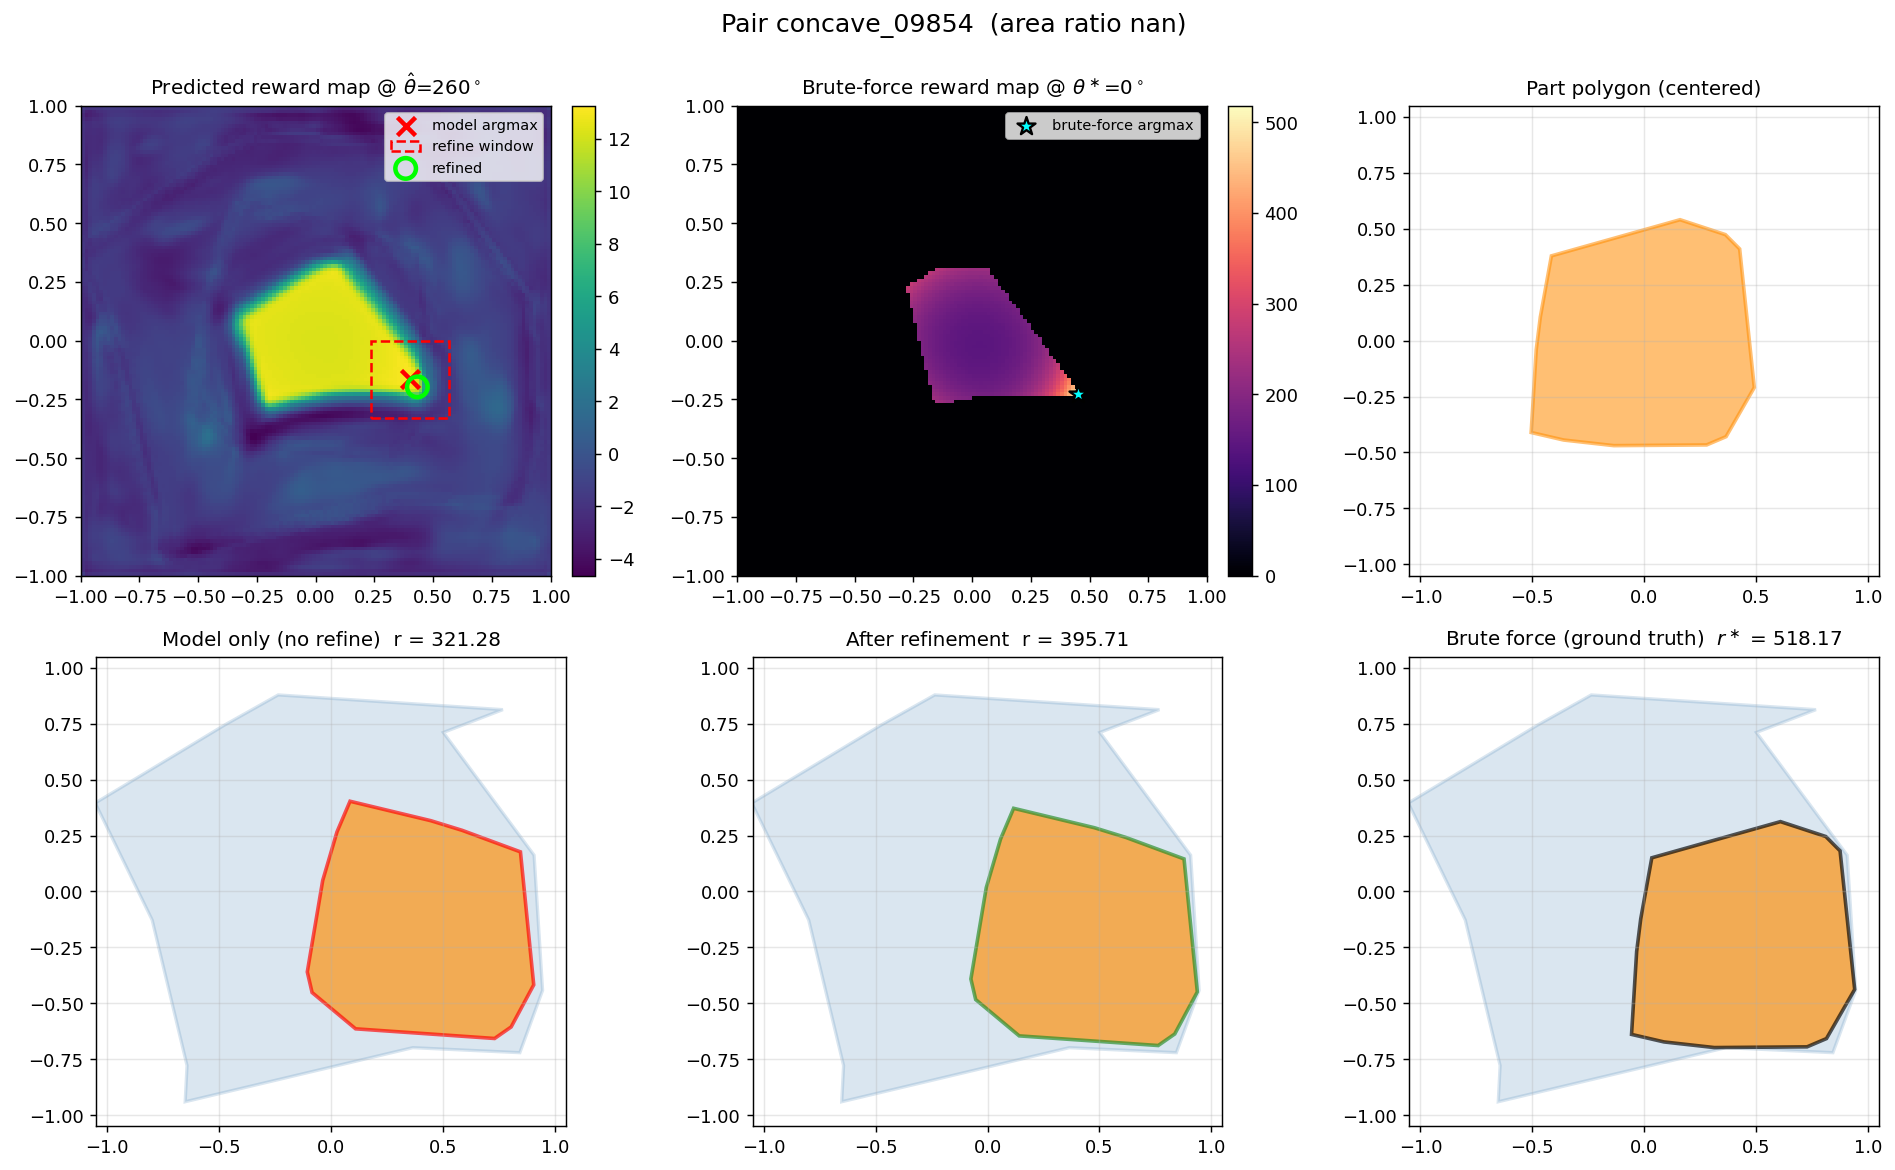
\includegraphics[width=\textwidth]{figs/concave_09854.png}
\end{figure}

\begin{center}\small
\begin{tabular}{lrrrr}
  \toprule
  Method & $\theta$ (deg) & $(x, y)$ & Reward & Recovery \\
  \midrule
  Brute force ($r^\ast$)    & 0 & $(+0.449, -0.228)$ & 518.172 & 1.000 \\
  Model only                & 260 & $(+0.402, -0.165)$       & 321.276 & 0.620 \\
  Refined ($\pm10$\,px, $\pm2$\,$\theta$-bins) & 260 & $(+0.433, -0.197)$ & 395.707 & 0.764 \\
  \bottomrule
\end{tabular}
\end{center}

\begin{center}\small
\begin{tabular}{lr}
  \toprule
  Cost & Value \\
  \midrule
  Rasterize (36 rotated part masks)              & 8.3 ms \\
  Model forward (36 passes, batched)             & 250.2 ms \\
  Shapely refinement (2205 calls, target 2205)  & 532.9 ms \\
  \midrule
  Total                                          & 791.4 ms \\
  \bottomrule
\end{tabular}
\end{center}

\section{Summary}

\begin{figure}[H]
\centering
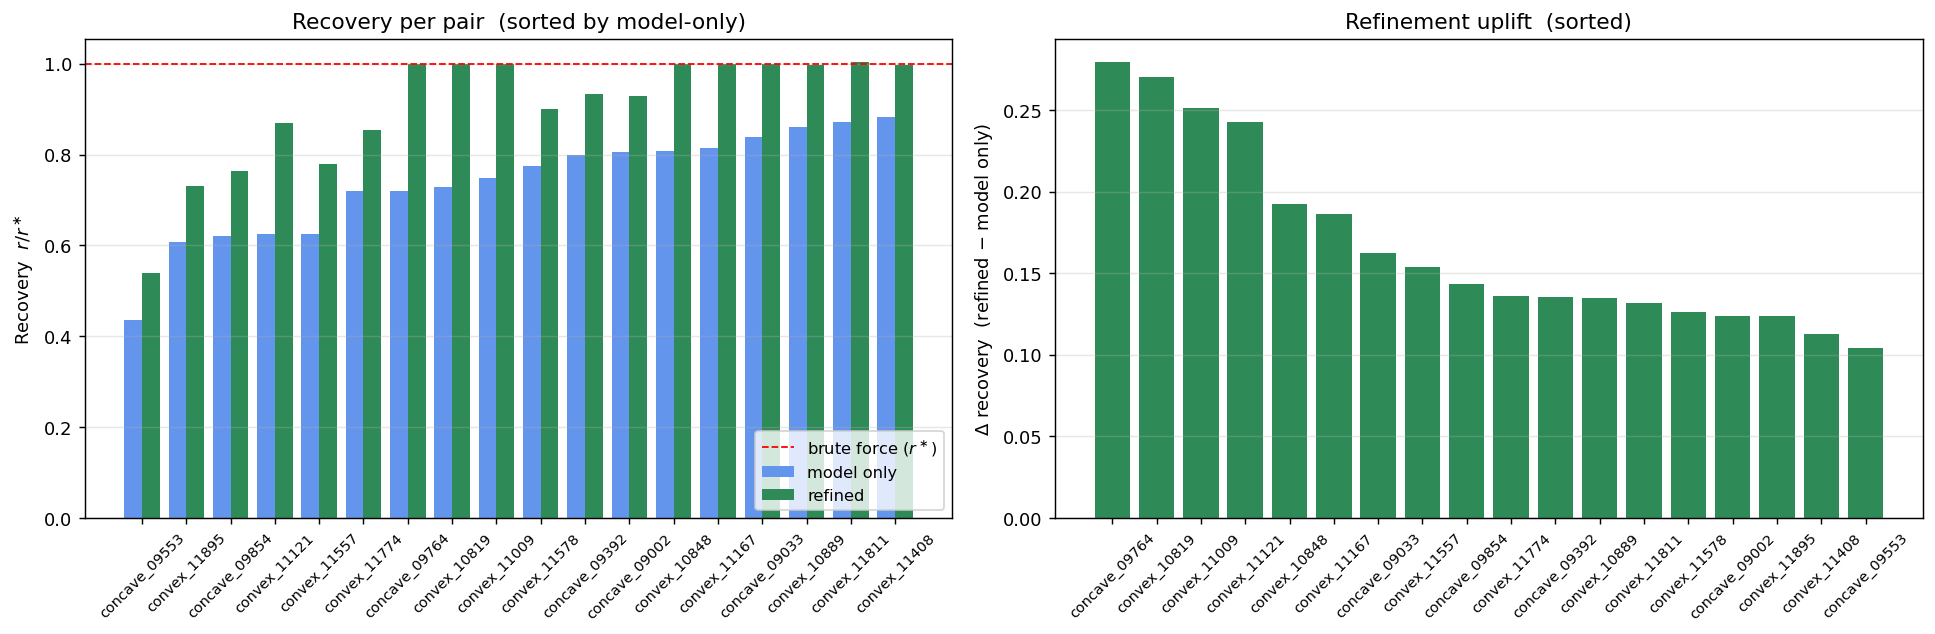
\includegraphics[width=\textwidth]{figs/summary.png}
\caption{Left: recovery $r / r^\ast$ per pair (model-only vs.\ refined). Right: refinement uplift sorted descending.}
\end{figure}

\begin{center}\small
\begin{tabular}{lr}
  \toprule
  Statistic & Value \\
  \midrule
  Pairs reported                          & 18 \\
  Mean recovery (model only)              & 0.7382 \\
  Mean recovery (refined)                 & 0.9054 \\
  Median recovery (model only)            & 0.7617 \\
  Median recovery (refined)               & 0.9652 \\
  Mean $\Delta$ recovery                  & +0.1672 \\
  Pairs where refinement helped           & 18/18 \\
  \midrule
  Mean time per pair (rasterize)          & 6.5 ms \\
  Mean time per pair (model forward)      & 212.3 ms \\
  Mean time per pair (refinement)         & 570.1 ms \\
  Mean Shapely calls per pair             & 2205 (expected 2205) \\
  \bottomrule
\end{tabular}
\end{center}

\end{document}
